%%%%%%%%%%%%%%%%%%%%%%%%%%%%%%%%%%%%%%%%%%%%%%%%%%%%%%%%%%%%%%%%%%%%%%
% Template for a UBC-compliant dissertation
% At the minimum, you will need to change the information found
% after the "Document meta-data"
%
%!TEX TS-program = pdflatex
%!TEX encoding = UTF-8 Unicode

%% The ubcdiss class provides several options:
%%   gpscopy (aka fogscopy)
%%       set parameters to exactly how GPS specifies
%%         * single-sided
%%         * page-numbering starts from title page
%%         * the lists of figures and tables have each entry prefixed
%%           with 'Figure' or 'Table'
%%       This can be tested by `\ifgpscopy ... \else ... \fi'
%%   10pt, 11pt, 12pt
%%       set default font size
%%   oneside, twoside
%%       whether to format for single-sided or double-sided printing
%%   balanced
%%       when double-sided, ensure page content is centred
%%       rather than slightly offset (the default)
%%   singlespacing, onehalfspacing, doublespacing
%%       set default inter-line text spacing; the ubcdiss class
%%       provides \textspacing to revert to this configured spacing
%%   draft
%%       disable more intensive processing, such as including
%%       graphics, etc.
%%

% For submission to GPS
\documentclass[gpscopy,onehalfspacing,11pt]{ubcdiss}

% For your own copies (looks nicer)
% \documentclass[balanced,twoside,11pt]{ubcdiss}

%%%%%%%%%%%%%%%%%%%%%%%%%%%%%%%%%%%%%%%%%%%%%%%%%%%%%%%%%%%%%%%%%%%%%%
%%%%%%%%%%%%%%%%%%%%%%%%%%%%%%%%%%%%%%%%%%%%%%%%%%%%%%%%%%%%%%%%%%%%%%
%%
%% FONTS:
%% 
%% The defaults below configures Times Roman for the serif font,
%% Helvetica for the sans serif font, and Courier for the
%% typewriter-style font.  Configuring fonts can be time
%% consuming; we recommend skipping to END FONTS!
%% 
%% If you're feeling brave, have lots of time, and wish to use one
%% your platform's native fonts, see the commented out bits below for
%% XeTeX/XeLaTeX.  This is not for the faint at heart. 
%% (And shouldn't you be writing? :-)
%%

%% NFSS font specification (New Font Selection Scheme)
\usepackage{times,mathptmx,courier}
\usepackage[scaled=.92]{helvet}

%% Math or theory people may want to include the handy AMS macros
\usepackage{amssymb}
\usepackage{amsmath}
\usepackage{amsfonts}

%% The pifont package provides access to the elements in the dingbat font.   
%% Use \ding{##} for a particular dingbat (see p7 of psnfss2e.pdf)
%%   Useful:
%%     51,52 different forms of a checkmark
%%     54,55,56 different forms of a cross (saltyre)
%%     172-181 are 1-10 in open circle (serif)
%%     182-191 are 1-10 black circle (serif)
%%     192-201 are 1-10 in open circle (sans serif)
%%     202-211 are 1-10 in black circle (sans serif)
%% \begin{dinglist}{##}\item... or dingautolist (which auto-increments)
%% to create a bullet list with the provided character.
\usepackage{pifont}

%%%%%%%%%%%%%%%%%%%%%%%%%%%%%%%%%%%%%%%%%%%%%%%%%%%%%%%%%%%%%%%%%%%%%%
%% Configure fonts for XeTeX / XeLaTeX using the fontspec package.
%% Be sure to check out the fontspec documentation.
%\usepackage{fontspec,xltxtra,xunicode}	% required
%\defaultfontfeatures{Mapping=tex-text}	% recommended
%% Minion Pro and Myriad Pro are shipped with some versions of
%% Adobe Reader.  Adobe representatives have commented that these
%% fonts can be used outside of Adobe Reader.
%\setromanfont[Numbers=OldStyle]{Minion Pro}
%\setsansfont[Numbers=OldStyle,Scale=MatchLowercase]{Myriad Pro}
%\setmonofont[Scale=MatchLowercase]{Andale Mono}

%% Other alternatives:
%\setromanfont[Mapping=tex-text]{Adobe Caslon}
%\setsansfont[Scale=MatchLowercase]{Gill Sans}
%\setsansfont[Scale=MatchLowercase,Mapping=tex-text]{Futura}
%\setmonofont[Scale=MatchLowercase]{Andale Mono}
%\newfontfamily{\SYM}[Scale=0.9]{Zapf Dingbats}
%% END FONTS
%%%%%%%%%%%%%%%%%%%%%%%%%%%%%%%%%%%%%%%%%%%%%%%%%%%%%%%%%%%%%%%%%%%%%%
%%%%%%%%%%%%%%%%%%%%%%%%%%%%%%%%%%%%%%%%%%%%%%%%%%%%%%%%%%%%%%%%%%%%%%



%%%%%%%%%%%%%%%%%%%%%%%%%%%%%%%%%%%%%%%%%%%%%%%%%%%%%%%%%%%%%%%%%%%%%%
%%%%%%%%%%%%%%%%%%%%%%%%%%%%%%%%%%%%%%%%%%%%%%%%%%%%%%%%%%%%%%%%%%%%%%
%%
%% Recommended packages
%%
\usepackage{checkend}	% better error messages on left-open environments
\usepackage{graphicx}	% for incorporating external images

%% booktabs: provides some special commands for typesetting tables as used
%% in excellent journals.  Ignore the examples in the Lamport book!
\usepackage{booktabs}

%% listings: useful support for including source code listings, with
%% optional special keyword formatting.  The \lstset{} causes
%% the text to be typeset in a smaller sans serif font, with
%% proportional spacing.
\usepackage{listings}
\lstset{basicstyle=\sffamily\scriptsize,showstringspaces=false,fontadjust}

%% The acronym package provides support for defining acronyms, providing
%% their expansion when first used, and building glossaries.  See the
%% example in glossary.tex and the example usage throughout the example
%% document.
%% NOTE: to use \MakeTextLowercase in the \acsfont command below,
%%   we *must* use the `nohyperlinks' option -- it causes errors with
%%   hyperref otherwise.  See Section 5.2 in the ``LaTeX 2e for Class
%%   and Package Writers Guide'' (clsguide.pdf) for details.
\usepackage[printonlyused,nohyperlinks]{acronym}
%% The ubcdiss.cls loads the `textcase' package which provides commands
%% for upper-casing and lower-casing text.  The following causes
%% the acronym package to typeset acronyms in small-caps
%% as recommended by Bringhurst.
\renewcommand{\acsfont}[1]{{\scshape \MakeTextLowercase{#1}}}

%% color: add support for expressing colour models.  Grey can be used
%% to great effect to emphasize other parts of a graphic or text.
%% For an excellent set of examples, see Tufte's "Visual Display of
%% Quantitative Information" or "Envisioning Information".
\usepackage{color}
\definecolor{greytext}{gray}{0.5}

%% comment: provides a new {comment} environment: all text inside the
%% environment is ignored.
%%   \begin{comment} ignored text ... \end{comment}
\usepackage{comment}

%% The natbib package provides more sophisticated citing commands
%% such as \citeauthor{} to provide the author names of a work,
%% \citet{} to produce an author-and-reference citation,
%% \citep{} to produce a parenthetical citation.
%% We use \citeeg{} to provide examples
\usepackage[numbers,sort&compress]{natbib}
\newcommand{\citeeg}[1]{\citep[e.g.,][]{#1}}

%% The titlesec package provides commands to vary how chapter and
%% section titles are typeset.  The following uses more compact
%% spacings above and below the title.  The titleformat that follow
%% ensure chapter/section titles are set in singlespace.
\usepackage[compact]{titlesec}
\titleformat*{\section}{\singlespacing\raggedright\bfseries\Large}
\titleformat*{\subsection}{\singlespacing\raggedright\bfseries\large}
\titleformat*{\subsubsection}{\singlespacing\raggedright\bfseries}
\titleformat*{\paragraph}{\singlespacing\raggedright\itshape}

%% The caption package provides support for varying how table and
%% figure captions are typeset.
\usepackage[format=hang,indention=-1cm,labelfont={bf},margin=1em]{caption}

%% url: for typesetting URLs and smart(er) hyphenation.
%% \url{http://...} 
\usepackage{url}
\urlstyle{sf}	% typeset urls in sans-serif

%%%%%%%%%%%%%%%%%%%%%%%%%%%%%%%%%%%%%%%%%%%%%%%%%%%%%%%%%%%%%%%%%%%%%%
%%%%%%%%%%%%%%%%%%%%%%%%%%%%%%%%%%%%%%%%%%%%%%%%%%%%%%%%%%%%%%%%%%%%%%
\usepackage{xcolor}
\usepackage{multirow}
\usepackage{pdflscape}

\usepackage{mdframed}
\usepackage{ntheorem}

\theoremstyle{nonumberplain}
\newmdtheoremenv{summary}{Summary}

%%%%%%%%%%%%%%%%%%%%%%%%%%%%%%%%%%%%%%%%%%%%%%%%%%%%%%%%%%%%%%%%%%%%%%
%%%%%%%%%%%%%%%%%%%%%%%%%%%%%%%%%%%%%%%%%%%%%%%%%%%%%%%%%%%%%%%%%%%%%%
%%
%% Possibly useful packages: you may need to explicitly install
%% these from CTAN if they aren't part of your distribution;
%% teTeX seems to ship with a smaller base than MikTeX and MacTeX.
%%
\usepackage{pdfpages}	% insert pages from other PDF files
%\usepackage{longtable}	% provide tables spanning multiple pages
%\usepackage{chngpage}	% support changing the page widths on demand
\usepackage{tabularx}	% an enhanced tabular environment

%% enumitem: support pausing and resuming enumerate environments.
\usepackage{enumitem}

%% rotating: provides two environments, sidewaystable and sidewaysfigure,
%% for typesetting tables and figures in landscape mode.  
%\usepackage{rotating}

%% subfig: provides for including subfigures within a figure,
%% and includes being able to separately reference the subfigures.
\usepackage{subfig}

%% ragged2e: provides several new new commands \Centering, \RaggedLeft,
%% \RaggedRight and \justifying and new environments Center, FlushLeft,
%% FlushRight and justify, which set ragged text and are easily
%% configurable to allow hyphenation.
\usepackage{ragged2e}

%% The ulem package provides a \sout{} for striking out text and
%% \xout for crossing out text.  The normalem and normalbf are
%% necessary as the package messes with the emphasis and bold fonts
%% otherwise.
%\usepackage[normalem,normalbf]{ulem}    % for \sout

%%%%%%%%%%%%%%%%%%%%%%%%%%%%%%%%%%%%%%%%%%%%%%%%%%%%%%%%%%%%%%%%%%%%%%
%% HYPERREF:
%% The hyperref package provides for embedding hyperlinks into your
%% document.  By default the table of contents, references, citations,
%% and footnotes are hyperlinked.
%%
%% Hyperref provides a very handy command for doing cross-references:
%% \autoref{}.  This is similar to \ref{} and \pageref{} except that
%% it automagically puts in the *type* of reference.  For example,
%% referencing a figure's label will put the text `Figure 3.4'.
%% And the text will be hyperlinked to the appropriate place in the
%% document.
%%
%% Generally hyperref should appear after most other packages

%% The `pagebackref' causes the references in the bibliography to have
%% back-references to the citing page; `backref' puts the citing section
%% number.  See further below for other examples of using hyperref.
%% 2009/12/09: now use `linktocpage' (Jacek Kisynski): GPS now prefers
%%   that the ToC, LoF, LoT place the hyperlink on the page number,
%%   rather than the entry text.
\ifgpscopy
  % GPS requires that weblinks should be dark blue, which looks a bit
  % odd in printed form.
  % https://www.grad.ubc.ca/current-students/dissertation-thesis-preparation/fonts-print
  \usepackage[bookmarks,bookmarksnumbered,%
     pagebackref,linktocpage,%
     colorlinks=true,%
     linkcolor=black,%
     urlcolor=blue,%
     citecolor=black%
     ]{hyperref}
\else
  %% The following puts hyperlinks in very faint grey boxes (in pdf only).
  \usepackage[bookmarks,bookmarksnumbered,%
    pagebackref,linktocpage,%
    allbordercolors={0.8 0.8 0.8},%
    ]{hyperref}
\fi
%% The following change how the the back-references text is typeset in a
%% bibliography when `backref' or `pagebackref' are used
%%
%% Change \nocitations if you'd like some text shown where there
%% are no citations found (e.g., pulled in with \nocite{xxx})
\newcommand{\nocitations}{\relax}
%%\newcommand{\nocitations}{No citations}
%%
%\renewcommand*{\backref}[1]{}% necessary for backref < 1.33
\renewcommand*{\backrefsep}{,~}%
\renewcommand*{\backreftwosep}{,~}% ', and~'
\renewcommand*{\backreflastsep}{,~}% ' and~'
\renewcommand*{\backrefalt}[4]{%
\textcolor{greytext}{\ifcase #1%
\nocitations%
\or
\(\rightarrow\) page #2%
\else
\(\rightarrow\) pages #2%
\fi}}


%% The following uses most defaults, which causes hyperlinks to be
%% surrounded by colourful boxes; the colours are only visible in
%% PDFs and don't show up when printed:
%\usepackage[bookmarks,bookmarksnumbered]{hyperref}

%% The following disables the colourful boxes around hyperlinks.
%\usepackage[bookmarks,bookmarksnumbered,pdfborder={0 0 0}]{hyperref}

%% The following disables all hyperlinking, but still enabled use of
%% \autoref{}
%\usepackage[draft]{hyperref}

%% The following commands causes chapter and section references to
%% uppercase the part name.
\renewcommand{\chapterautorefname}{Chapter}
\renewcommand{\sectionautorefname}{Section}
\renewcommand{\subsectionautorefname}{Section}
\renewcommand{\subsubsectionautorefname}{Section}

%% If you have long page numbers (e.g., roman numbers in the 
%% preliminary pages for page 28 = xxviii), you might need to
%% uncomment the following and tweak the \@pnumwidth length
%% (default: 1.55em).  See the tocloft documentation at
%% http://www.ctan.org/tex-archive/macros/latex/contrib/tocloft/
% \makeatletter
% \renewcommand{\@pnumwidth}{3em}
% \makeatother

%%%%%%%%%%%%%%%%%%%%%%%%%%%%%%%%%%%%%%%%%%%%%%%%%%%%%%%%%%%%%%%%%%%%%%
%%%%%%%%%%%%%%%%%%%%%%%%%%%%%%%%%%%%%%%%%%%%%%%%%%%%%%%%%%%%%%%%%%%%%%
%%
%% Some special settings that controls how text is typeset
%%
% \raggedbottom		% pages don't have to line up nicely on the last line
% \sloppy		% be a bit more relaxed in inter-word spacing
% \clubpenalty=10000	% try harder to avoid orphans
% \widowpenalty=10000	% try harder to avoid widows
% \tolerance=1000

%% And include some of our own useful macros
% This file provides examples of some useful macros for typesetting
% dissertations.  None of the macros defined here are necessary beyond
% for the template documentation, so feel free to change, remove, and add
% your own definitions.
%
% We recommend that you define macros to separate the semantics
% of the things you write from how they are presented.  For example,
% you'll see definitions below for a macro \file{}: by using
% \file{} consistently in the text, we can change how filenames
% are typeset simply by changing the definition of \file{} in
% this file.
% 
%% The following is a directive for TeXShop to indicate the main file
%%!TEX root = diss.tex

\newcommand{\NA}{\textsc{n/a}}	% for "not applicable"
\newcommand{\eg}{e.g.,\ }	% proper form of examples (\eg a, b, c)
\newcommand{\ie}{i.e.,\ }	% proper form for that is (\ie a, b, c)
\newcommand{\etc}{etc.\ }
\newcommand{\etal}{et al. }
\newcommand{\sic}{\ [sic]\ }

% Some useful macros for typesetting terms.
\newcommand{\file}[1]{\texttt{#1}}
\newcommand{\class}[1]{\texttt{#1}}
\newcommand{\code}[1]{\texttt{#1}}
\newcommand{\commit}[1]{\texttt{#1}}
\newcommand{\entity}[1]{\textsc{#1}}
\newcommand{\jira}[2]{{\small \textsf{\textbf{#1}} \textsf{#2}}}
\newcommand{\latexpackage}[1]{\href{http://www.ctan.org/macros/latex/contrib/#1}{\texttt{#1}}}
\newcommand{\latexmiscpackage}[1]{\href{http://www.ctan.org/macros/latex/contrib/misc/#1.sty}{\texttt{#1}}}
\newcommand{\env}[1]{\texttt{#1}}
\newcommand{\BibTeX}{Bib\TeX}

% For making `\autoref` work with subfloats
\newcommand{\subfigureautorefname}{\figureautorefname}

% Define a command \doi{} to typeset a digital object identifier (DOI).
% Note: if the following definition raise an error, then you likely
% have an ancient version of url.sty.  Either find a more recent version
% (3.1 or later work fine) and simply copy it into this directory,  or
% comment out the following two lines and uncomment the third.
\DeclareUrlCommand\DOI{}
\newcommand{\doi}[1]{\href{http://dx.doi.org/#1}{\DOI{doi:#1}}}
%\newcommand{\doi}[1]{\href{http://dx.doi.org/#1}{doi:#1}}

% Useful macro to reference an online document with a hyperlink
% as well with the URL explicitly listed in a footnote
% #1: the URL
% #2: the anchoring text
\newcommand{\webref}[2]{\href{#1}{#2}\footnote{\url{#1}}}

% epigraph is a nice environment for typesetting quotations
\makeatletter
\newenvironment{epigraph}{%
	\begin{flushright}
	\begin{minipage}{\columnwidth-0.75in}
	\begin{flushright}
	\@ifundefined{singlespacing}{}{\singlespacing}%
    }{
	\end{flushright}
	\end{minipage}
	\end{flushright}}
\makeatother

% \FIXME{} is a useful macro for noting things needing to be changed.
% The following definition will also output a warning to the console
\newcommand{\FIXME}[1]{\typeout{**FIXME** #1}\textbf{[FIXME: #1]}}

% END


%%%%%%%%%%%%%%%%%%%%%%%%%%%%%%%%%%%%%%%%%%%%%%%%%%%%%%%%%%%%%%%%%%%%%%
%%%%%%%%%%%%%%%%%%%%%%%%%%%%%%%%%%%%%%%%%%%%%%%%%%%%%%%%%%%%%%%%%%%%%%
%%
%% Document meta-data: be sure to also change the \hypersetup information
%%

\title{Reducing the Cognitive and Temporal Costs of Software History Exploration}
%\subtitle{If you want a subtitle}

\author{Alison Li}
\previousdegree{B.A., McGill University, 2020}

% What is this dissertation for?
\degreetitle{Master of Science}

\institution{The University of British Columbia}
\campus{Vancouver}

\faculty{The Faculty of Science}
\department{Computer Science}
\submissionmonth{August}
\submissionyear{2022}

% details of your examining committee
\examiningcommittee{Gail C. Murphy, Computer Science}{Supervisor}
\examiningcommittee{Ryan Reynolds, Computer Science}%
    {Supervisory Committee Member}

% details of your supervisory committee
% \supervisorycommittee{Ira Crater, Materials Engineering}%
%     {Supervisory Committee Member}
% \supervisorycommittee{Adeline Long, \textsc{CEO} of Aerial Machine
%     Transportation, Inc.}{Supervisory Committee Member}

%% hyperref package provides support for embedding meta-data in .PDF
%% files
\hypersetup{
  pdftitle={Thesis  (DRAFT: \today)},
  pdfauthor={Alison Li},
  pdfkeywords={thesis}
}

%%%%%%%%%%%%%%%%%%%%%%%%%%%%%%%%%%%%%%%%%%%%%%%%%%%%%%%%%%%%%%%%%%%%%%
%%%%%%%%%%%%%%%%%%%%%%%%%%%%%%%%%%%%%%%%%%%%%%%%%%%%%%%%%%%%%%%%%%%%%%
%% 
%% The document content
%%

%% LaTeX's \includeonly commands causes any uses of \include{} to only
%% include files that are in the list.  This is helpful to produce
%% subsets of your thesis (e.g., for committee members who want to see
%% the dissertation chapter by chapter).  It also saves time by 
%% avoiding reprocessing the entire file.
%\includeonly{intro,conclusions}
%\includeonly{discussion}

\begin{document}

%%%%%%%%%%%%%%%%%%%%%%%%%%%%%%%%%%%%%%%%%%%%%%%%%%
%% From Thesis Components: Tradtional Thesis
%% <http://www.grad.ubc.ca/current-students/dissertation-thesis-preparation/order-components>

% Preliminary Pages (numbered in lower case Roman numerals)
%    1. Title page (mandatory)
\maketitle

%    2. Committee page (mandatory): lists supervisory committee and,
%    if applicable, the examining committee
\makecommitteepage

%    3. Abstract (mandatory - maximum 350 words)
%% The following is a directive for TeXShop to indicate the main file
%%!TEX root = diss.tex

\chapter{Abstract}

The abstract is a concise and accurate summary of the scholarly work described in the document. 
It states the problem, the methods of investigation, and the general conclusions, and should not contain tables, graphs, 
complex equations, or illustrations. 
There is a single scholarly abstract for the entire work, and it must not exceed 350 words in length.

% Consider placing version information if you circulate multiple drafts
%\vfill
%\begin{center}
%\begin{sf}
%\fbox{Revision: \today}
%\end{sf}
%\end{center}

\cleardoublepage

%    4. Lay Summary (Effective May 2017, mandatory - maximum 150 words)
%% The following is a directive for TeXShop to indicate the main file
%%!TEX root = diss.tex

%% https://www.grad.ubc.ca/current-students/dissertation-thesis-preparation/preliminary-pages
%% 
%% LAY SUMMARY Effective May 2017, all theses and dissertations must
%% include a lay summary.  The lay or public summary explains the key
%% goals and contributions of the research/scholarly work in terms that
%% can be understood by the general public. It must not exceed 150
%% words in length.

\chapter{Lay Summary}

This thesis investigates how identifying non-important and important 
revisions in a software system's revision history can help 
software developers to better answer questions about the motivation behind code.
Developers also may use issues, which are non-code artifacts tied to revisions, 
as a source of code rationale information.
\rev{To better support developers in exploring software history, 
we introduce a plugin for IntelliJ IDEA that consists of two approaches.}
\rev{The first approach} uses the lines of code changes in a revision
to determine if the revision solely contains code changes that the developer
might consider as non-essential.
\rev{The second approach} attempts to reduce context switching between an \entity{IDE}
and an application for viewing issue information, providing the developer with
better access to an issue along with other metrics about the issue.
To evaluate the plugin, we deployed a controlled laboratory study.
We collected data from a total of 10 software developers.
\cleardoublepage

%    5. Preface
%% The following is a directive for TeXShop to indicate the main file
%%!TEX root = diss.tex

\chapter{Preface}

The work presented in this thesis was conducted in the Software Practices Laboratory at the University of British Columbia, Point Grey campus.
All projects and associated methods were approved by the University of British Columbia's Research Ethics Board [certificate \#H22-01342].

I was the lead investigator, responsible for concept formation, implementation, data collection, analysis of the results, and manuscript composition.
Gail Murphy was the supervisory author on this project and was involved throughout concept formation and manuscript composition.

%%%%%%%%%%%%%%%%%%%%%%%%%%%%%%%%%%%%%%%%%%%%%%%%%%%%%%%%%%%%%%%%%%%%%%
\endinput

The Preface must include a statement indicating the student's contribution to the following:

\begin{itemize}
    \item Identification and design of the research program,
    \item Performance of the various parts of the research, and
    \item Analysis of the research data.
    \item Certain additional elements may also be required, as specified below.
\end{itemize}

If any of the work presented in the thesis has led to any publications or submissions, all of these must be listed in the Preface. 
Bibliographic details should include the title of the article and the name of the publisher (ONLY if the article has been accepted or published), and the chapter(s) of the thesis in which the associated work is located.
If the work includes publications or material submitted for publication, the statement described above must detail the relative contributions of all collaborators and co-authors (including supervisors and members of the supervisory committee) and state the proportion of research and writing conducted by the student. For further details, see “Including Published Material in a Thesis or Dissertation”.
If the work includes other scholarly artifacts (such as film and other audio, visual, and graphic representations, and application-oriented documents such as policy briefs, curricula, business plans, computer and web tools, pages, and applications, etc.), all of these must be listed in the Preface (with bibliographical information, if applicable).
If ethics approval was required for the research, the Preface must list the Certificate Number(s) of the Ethics Certificate(s) applicable to the project.
In a thesis where the research was not subject to ethics review, produced no publications, and was designed, carried out, and analyzed by the student alone, the text of the Preface may be very brief. Samples are available on this website and in the University Library's online repository of accepted theses.

The content of the Preface must be verified by the student's supervisor, whose endorsement must appear on the final Thesis/Dissertation Approval form.
\cleardoublepage

%    6. Table of contents (mandatory - list all items in the preliminary pages
%    starting with the abstract, followed by chapter headings and
%    subheadings, bibliographies and appendices)
\tableofcontents
\cleardoublepage	% required by tocloft package

%    7. List of tables (mandatory if thesis has tables)
\listoftables
\cleardoublepage	% required by tocloft package

%    8. List of figures (mandatory if thesis has figures)
\listoffigures
\cleardoublepage	% required by tocloft package

%    9. List of illustrations (mandatory if thesis has illustrations)
%   10. Lists of symbols, abbreviations or other (optional)

%   11. Glossary (optional)
%%% The following is a directive for TeXShop to indicate the main file
%%!TEX root = diss.tex

\chapter{Glossary}

% This glossary uses the handy \latexpackage{acroynym} package to automatically
% maintain the glossary.  It uses the package's \texttt{printonlyused}
% option to include only those acronyms explicitly referenced in the
% \LaTeX\ source.  To change how the acronyms are rendered, change the
% \verb+\acsfont+ definition in \verb+diss.tex+.

% use \acrodef to define an acronym, but no listing
\acrodef{UI}{user interface}
\acrodef{UBC}{University of British Columbia}

% The acronym environment will typeset only those acronyms that were
% *actually used* in the course of the document
\begin{acronym}[ANOVA]
\acro{ANOVA}[ANOVA]{Analysis of Variance\acroextra{, a set of
  statistical techniques to identify sources of variability between groups}}
\acro{API}{application programming interface}
\acro{CTAN}{\acroextra{The }Common \TeX\ Archive Network}
\acro{DOI}{Document Object Identifier\acroextra{ (see
    \url{http://doi.org})}}
\acro{GPS}[GPS]{Graduate and Postdoctoral Studies}
\acro{PDF}{Portable Document Format}
\acro{RCS}[RCS]{Revision control system\acroextra{, a software
    tool for tracking changes to a set of files}}
\acro{TLX}[TLX]{Task Load Index\acroextra{, an instrument for gauging
  the subjective mental workload experienced by a human in performing
  a task}}
\acro{UML}{Unified Modelling Language\acroextra{, a visual language
    for modelling the structure of software artefacts}}
\acro{URL}{Unique Resource Locator\acroextra{, used to describe a
    means for obtaining some resource on the world wide web}}
\acro{W3C}[W3C]{\acroextra{the }World Wide Web Consortium\acroextra{,
    the standards body for web technologies}}
\acro{XML}{Extensible Markup Language}
\acro{API}{Application Programming Interface}
\acro{IDE}{Integrated Development Environment}
\end{acronym}

% You can also use \newacro{}{} to only define acronyms
% but without explictly creating a glossary
% 
% \newacro{ANOVA}[ANOVA]{Analysis of Variance\acroextra{, a set of
%   statistical techniques to identify sources of variability between groups.}}
% \newacro{API}[API]{application programming interface}
% \newacro{GOMS}[GOMS]{Goals, Operators, Methods, and Selection\acroextra{,
%   a framework for usability analysis.}}
% \newacro{TLX}[TLX]{Task Load Index\acroextra{, an instrument for gauging
%   the subjective mental workload experienced by a human in performing
%   a task.}}
% \newacro{UI}[UI]{user interface}
% \newacro{UML}[UML]{Unified Modelling Language}
% \newacro{W3C}[W3C]{World Wide Web Consortium}
% \newacro{XML}[XML]{Extensible Markup Language}
	% always input, since other macros may rely on it

\textspacing		% begin one-half or double spacing

%   12. Acknowledgements (optional)
%%% The following is a directive for TeXShop to indicate the main file
%%!TEX root = diss.tex

\chapter{Acknowledgments}

I am incredibly fortunate to have had the opportunity to be supervised by Gail Murphy,
and to have had her support and encouragement that allowed me to pursue the work in this thesis.
This work would not have been possible without her.

I am grateful to Ed Knorr, who provided thorough feedback as the second reader to this thesis,
and who was also an excellent instructor in the brief period I served as a \entity{TA} for him.

I am also thankful for all of the participants who were involved in the evaluation of the work presented in this thesis
and provided interesting insights into their habits and perspectives as developers.

Lastly, I thank my mother for her unwavering and unconditional emotional and financial support for me and my education.

As I grow older, I increasingly cherish the value of time as a finite resource.
To all of the individuals, both stated above and beyond in my life,
I cannot thank you enough for the time you have generously given me in helping to produce and present the work in this thesis.

%   13. Dedication (optional)

% Body of Thesis (not all sections may apply)
\mainmatter

\acresetall	% reset all acronyms used so far

%    1. Introduction
%% This is the original intro.tex file. 
%% The following is a directive for TeXShop to indicate the main file
%%!TEX root = diss.tex

\chapter{Introduction}
\label{ch:Introduction}

%%%%%%%%%%%%%%%%%%%%%%%%%%%%%%%%%%%%%%%%%%%%%%%%%%%%%%%%%%%%%%%%%%%%%%

Rarely does a developer join a team at the inception of a code base. 
This being the case, developers navigating a team's source code for the first time often ask the question: ``why was this code written this way?'' inquiring about the motivations behind the code left by former and current colleagues.
LaToza \etal found the most serious problem software developers face is understanding code rationale \cite{latoza_maintaining_2006}.
In agreement, Ko \etal report that finding the intent behind code is the most difficult information need to satisfy \cite{ko_information_2007}. 
In further agreement, LaToza and Myers unearth code rationale as the single most frequently reported “hard-to-answer” question category in software development \cite{latoza_hard-answer_2010}. 
Code rationale includes questions not clearly answered by examining code itself, such as algorithm choice, optimization choice, and hidden criteria that motivate design choices \cite{latoza_hard-answer_2010}. 
One common information source LaToza \etal report on is colleagues. 
However, the practice of seeking knowledgeable colleagues is challenging in projects experiencing turnover. 
In the context of colleague turnover, LaToza et al.'s assertion of the existence of a quintessential ``team historian'' in a software development team \cite{latoza_maintaining_2006} becomes wishful thinking:

\begin{quote}
Almost all teams have a team historian who is the go-to person for questions about the
code. Often this person is the developer lead and has been with the code base the longest.
\end{quote}

What does one do when such a historian does not exist in a team? Or when a team experiences turnover?
There is a danger in relying solely on individuals for knowledge on intent behind the code in a large software system.
Confronted with turnover-induced knowledge loss, Robillard emphasizes developers leveraging artifacts from project history after a colleague’s departure to understand developer intent behind code a departed colleague wrote \cite{robillard_turnover-induced_2021}. 
However, developers often choose to forego investigating design documents due to the difficulties and cost of locating them \cite{latoza_maintaining_2006}.
It therefore becomes all the more important to reduce the cost for developers in using artifacts from a project's history to obtain code rationale. 

Project artifacts that can serve as a source for answering code rationale questions include: (1) revision history and (2) information from issue tracking systems (\entity{ITS}) or issue repositories. 
Developers investigate commit history to understand ``why is this [code] ‘this’ way'' as viewing code changes at points in time can help to recover the motivation behind segments of code.
In particular, investigating commit history can help a developer understand the evolution of source code, which is helpful for uncovering architectural patterns and decisions, requirements decisions, and frequently occurring bugs \cite{codoban_software_2015}.
Commits can also be accompanied by issues in a project issue repository. 
A typical practice in software development is to explicitly reference an issue ID from an \entity{ITS} in a commit message, where each commit is associated with an issue. 
Apache Kafka is one example of an open-source project, which uses this practice.\footnote{\url{https://kafka.apache.org/}, verified 3/7/2022.} \footnote{\url{https://kafka.apache.org/contributing}, verified 3/7/2022.}
For example: 

\begin{center}
	\jira{KAFKA-3715:}{Add granular metrics to Kafka Streams and add hierarhical \sic logging levels to Metrics}
\end{center}

\noindent is the title of one commit in the \class{KafkaStreams} class from the Apache Kafka repository.\footnote{\url{https://github.com/apache/kafka}, verified 7/20/2022.}
The bold portion identifies the key for the Jira issue associated with the commit, 
which can be viewed on the Apache Software Foundation's Jira instance.\footnote{\url{https://issues.apache.org/}, verified 3/7/2022.}

While commit history accessed from version control systems like Git provides information on lines of code changed at a point in time, 
the information from a commit's associated issue on an issue tracking platform 
such as Jira \cite{jira} can provide context around a commit through the issue's discussion, labels, number of developers subscribed, and priority among other aspects.
Through the commit history for a file and its linked Jira issues, 
we therefore get a change in time paired with a potential discussion or post at a point in time.
There are many tools that exist to explore commit history and manage the use of VCS. 
For example, \entity{git} ``blame'' \cite{gitblame}, graphical user interfaces such as Sourcetree \cite{sourcetree} and GitExtensions \cite{gitextensions}. 
Popular editors like Visual Studio Code \cite{vscode}, Eclipse \cite{eclipse}, and IntelliJ IDEA \cite{intellij} have native Git integrations and plugins that make the usage of Git more convenient and thereby make it easier to examine commits in a project's history. 
However, to the best of our knowledge, none of these tools provide support for easily gaining a synthesized view of the contents in a commit and the issue information associated with a commit.

Despite a wealth of tools supporting Git integration, Codoban et al.'s survey of 217 developers found 47\% of respondents reporting the high volume of commits in a project to be a challenge of navigating commit history \cite{codoban_software_2015}. 
Noise \eg white spaces, line-endings, and tangled commits make software history exploration inefficient. 
Ultimately, a developer still must manually identify meaningful commits, visit and read through the referenced issue, and maintain a mental model or narrative the developer constructs through a process of viewing code changes and keeping up with associated discussions that could provide the motivation for a code modification. 

%%%%%%%%%%%%%%%%%%%%%%%%%%%%%%%%%%%%%%%%%%%%%%%%%%%%%%%%%%%%%%%%%%%%%%

\section{Motivating Example}

We illustrate the cognitive and temporal burden of the process through a scenario.
Suppose \rev{a developer is new to} the open-source Apache Kafka project. 
Apache Kafka is an open-source streaming platform used for working with streaming data. 
Apache Kafka is most commonly used for real-time data processing and provides five core \entity{API}s: 
Producer, Consumer, Streams, Connect, and Admin.
Apache Kafka requires all non-trivial changes to have a corresponding Jira issue. 
\rev{The new developer is assigned the task to add support for configuring topologies in the Kafka \entity{API}.
Hence, the developer opens the file \file{Topology.java}.
To gain a sense of the changes that have taken place in the file,
which can help them determine if the file is relevant to the change they are tasked with making,
the developer is motivated to examine the commit history for the \class{Topology} class.}
In the context of the Kafka architecture, a ``topology'' is a directed acyclic graph of stream processing nodes 
that defines the stream processing logic for an application using Apache Kafka.
When viewing the commit history for the \class{Topology} class, the developer sees 22 commits.
The commit history in terms of the commit message subject for each commit is shown in \autoref{fig:Topology-Commit-History}.

To gain a sense of how \class{Topology} has evolved over time 
and for understanding the motivations behind code changes in the class, 
the developer manually inspects the diff between each of the 22 commits to understand 
how the code has evolved along different commit authors' intentions.
\rev{The developer encounters several commits 
that, at first glance, seem relevant for understanding the evolution of the \class{Topology} class.}
Despite some of these commits having commit message subjects that seem potentially 
meaningful, such as introducing the implementation of a feature, 
the developer finds they trivially affect the \class{Topology} class.
These commits are composed only of changes affecting documentation, annotations, imports, or newlines.
For example: 

\begin{center}
	\jira{KAFKA-7021:}{Reuse source based on config (\#5163)} (\commit{d98ec333})
\end{center}

\noindent describes largely fixing behaviours in other Kafka classes and adding unit tests for the fixed behaviour 
but insofar as \class{Topology} is concerned, the commit simply removes a newline, not impacting any behaviour in the class.

Another example is: 

\begin{center}
	\jira{KAFKA-5671:}{Add StreamsBuilder and Deprecate KStreamBuilder} (\commit{da220557})
\end{center}

\noindent which refactors several other class related to the Streams \entity{API} 
but in \class{Topology}, the commit only adds a missing \code{@param} tag 
to the documentation for the \code{addStateStore} method 
and adds documentation for the \code{describe} method.
Although changes that revise documentation could be useful for understanding evolution in class documentation, 
these types of changes could also be long outdated for the current state of the file 
and clutters the commit history that a developer skims when searching for code rationale related to present code.

In total, our heuristic-based approach, explained further in \autoref{sec:Heuristics}, 
shows 9 of 22 commits can be considered unimportant to the \class{Topology} class. 
We find 9 commits only affect documentation, annotations, and newlines.
If this were indicated in advance to the developer, this could have made the developer's search more efficient 
by considering the indication and have the choice to skip examining these commits.

\rev{Further, several of the messages for the commits contain insufficient information
for helping the developer understand the rationale behind the code changes in them.
For example, one commit has the message title:

\begin{center}
	\jira{KAFKA-10436:}{Implement KIP-478 Topology changes (\#9221)} (\commit{09d1498e})
\end{center}

\noindent where the body of the commit message states:

\begin{quote}
	\textsf{
		Convert Topology\#addProcessor and \#addGlobalStore
		\\ Also, convert some of the internals in support of addProcessor
	}
\end{quote}

\noindent which describes \emph{what} was changed in the commit but not \emph{why}.
Upon visiting the Jira issue, the developer is able to learn that
the commit adds type safety to the Processor \entity{API},
adding new \code{addProcessor} and \code{addGlobalStateStore} methods
to the \class{Topology} class to help enforce the introduction of the type safety enhancement.

As a result, while examining each commit, the developer constantly switches contexts between 
the view for examining \class{Topology}'s commit history 
and a view for visiting a commit's referenced Jira issue 
to gain more information about the motivation behind the code changed.
If the developer knew beforehand whether a commit's associated Jira issue
contained any additional insight on the rationale behind the change,
their search for rationale information to gain a better understanding
about the evolution of the file could be more efficient.}

In traversing the whole commit history for the \class{Topology} class,
the developer must maintain a mental model of the file's evolution 
and the rationale behind each change at different points in time. 
This results in a temporal cost of determining non-trivial commits to discard during exploration 
and a cognitive cost of maintaining a mental model of the interactions and decisions behind changes in a file.

%%%%%%%%%%%%%%%%%%%%%%%%%%%%%%%%%%%%%%%%%%%%%%%%%%%%%%%%%%%%%%%%%%%%%%

\section{Intelligent History}

This suggests the developer would benefit from an automatic and more streamlined approach to determining non-trivial commits to look at.
Additionally, the ability to glean the Jira issue information could help the developer more efficiently decide which commits they can prioritize exploring for understanding the evolution and rationale behind changes in the \class{Topology} class.
If such a tool could spotlight the remaining 13 of 22 commits to prioritize examining, the developer would be able to efficiently piece together the following about the \class{Topology} class. 
There were several refactoring commits: \jira{KAFKA-5670} is the first commit in the file and introduces \class{Topology} as a refactoring of a former class due to leakage of internal methods in the Kafka Streams \entity{API} that should not be public. 
The next commit \jira{KAFKA-5650} updates the \class{Topology} class to use newly added interfaces for reducing heavy method overloading.
Further commits \jira{KAFKA-12648} and \jira{KAFKA-12648} also explicitly state they refactor the \class{Topology} class to enable topology-specific user configuration.
Since these are refactoring commits, a tool could help to further optimize a developer's search by mitigating the need to visit the referenced Jira issues to find this out if it could provide the ability to glimpse the Jira issue descriptions or metrics that could measure a Jira's level of importance, \eg the number of people subscribed to a Jira issue.

If such a tool were available, the developer might be able to more easily see the more interesting changes and supporting rationale that occurred in \class{Topology}:
\jira{KAFKA-4936} addresses a previous limitation in the Kafka Streams \entity{API} where a stream's output topic had to be known prior, preventing the sending of output topics dynamically. 
The Jira description leads further to a link on open questions on topic creation and configuration in light of many requests to add the feature.
Similarly, \jira{KAFKA-7523} committed after describes another topology configuration-related shortcoming and adds support for state stores to each processor node in a topology.
These commits raise limitations in the Kafka Streams \entity{API} and user desire for more configuration support regarding topologies in Kafka, which lead to interesting discussion that a present developer viewing the history could read and understand as a historical concern surrounding the \class{Topology} class.

\begin{figure}
	\begin{mdframed}
	\begin{RaggedRight}
		\jira{KAFKA-9847:}{add config to set default store type (KIP-591) (\#11705)} \\
		\jira{KAFKA-12648:}{introduce TopologyConfig and TaskConfig for topology-level overrides (\#11272)} \\
		\textcolor{gray}{\jira{KAFKA-10546:}{Deprecate old PAPI (\#10869)}} \\
		\jira{KAFKA-12648:}{basic skeleton API for NamedTopology (\#10615)} \\
		\textcolor{gray}{\jira{KAFKA-10036:}{Improve handling and documentation of Suppliers (\#9000)}} \\
		\textcolor{gray}{\jira{MINOR:}{Clean-up streams javadoc warnings (\#9461)}} \\
		\textcolor{gray}{\jira{KAFKA-10605:}{Deprecate old PAPI registration methods (\#9448)}} \\
		\jira{KAFKA-10436:}{Implement KIP-478 Topology changes (\#9221)} \\
		\jira{KAFKA-10379:}{Implement the KIP-478 StreamBuilder\#addGlobalStore() (\#9148)} \\
		\jira{KAFKA-7523:}{Add ConnectedStoreProvider to Processor API (\#6824)} \\
		\jira{MINOR:}{Fix generic types in StreamsBuilder and Topology (\#8273)} \\
		\textcolor{gray}{\jira{KAFKA-6161}{Add default implementation to close() and configure() for Serdes (\#5348)}} \\
		\textcolor{gray}{\jira{MINOR:}{Return correct instance of SessionWindowSerde (\#5546)}} \\
		\textcolor{gray}{\jira{KAFKA-7021:}{Reuse source based on config (\#5163)}} \\
		\jira{KAFKA-4936:}{Add dynamic routing in Streams (\#5018)} \\
		\textcolor{gray}{\jira{MINOR:}{Add missing generics and surpress warning annotations (\#4518)}} \\
		\jira{MINOR:}{add suppress warnings annotations in Streams API} \\
		\textcolor{gray}{\jira{MINOR:}{JavaDoc improvements for new state store API}} \\
		\jira{KAFKA-5873;}{add materialized overloads to StreamsBuilder} \\
		\jira{KAFKA-5650;}{add StateStoreBuilder interface and implementations} \\
		\textcolor{gray}{\jira{KAFKA-5671:}{Add StreamsBuilder and Deprecate KStreamBuilder}} \\
		\jira{KAFKA-5670:}{(KIP-120) Add Topology and deprecate TopologyBuilder} \\
	\end{RaggedRight}
	\end{mdframed}
	\caption{The commit history, shown by each commit message's subject, for \class{Topology} class in the open-source Apache Kafka project. 
		The history is in descending order, from the most recent commit to the oldest commit.
		In total, \class{Topology} has 22 commits in its commit history. The greyed out commits contain changes deemed not meaningful due to being modifications only to documentation, annotations, imports, or newlines.
	}
	\label{fig:Topology-Commit-History}
\end{figure}

We hypothesize identifying important commits automatically and providing integrated access between commit 
and issue information could help a developer more effectively access the rationale for code.
This approach to presenting a commit history would reduce the cognitive and temporal costs of software history examination. 
This thesis investigates the design of \rev{an \entity{IDE} plugin} to spotlight potentially meaningful commits and de-emphasize 
less meaningful commits in the commit history for a file in a project and to make it more convenient 
to locate and access relevant issues referenced in a commit. 

%%%%%%%%%%%%%%%%%%%%%%%%%%%%%%%%%%%%%%%%%%%%%%%%%%%%%%%%%%%%%%%%%%%%%%

\section{Thesis Overview}

We develop a set of heuristics on code changes and Jira issues that for supporting a developer 
in gauging the relevance of commits and related Jira issues when seeking answers 
to code rationale questions pertaining to a file.
The design of the tool allows exploration of how effective the heuristics are 
for streamlining the process of viewing both commits and associated Jira issues in one interface, 
while also reducing the noise in a file's commit history.

We anticipate this approach will make it more convenient for a developer to gain insight into the evolution of code in a file that can further help to answer questions about the rationale behind the different changes in its evolution. 
For example, with de-emphasis on trivial commits in a file's commit history, a user might be able to see more clearly which commits introduced features in a file and which commits in between feature introductions were bug fixes or updates to a feature.
A developer who is new to a particular section of the code base that the file belongs to could then gain an understanding of any trends or historical bugs in that file, 
or discussions from previous developers who might have foreseen future problems related to existing implementation in the file.

To evaluate the effectiveness of our approach towards our hypothesis, 
we present Intelligent History, a plugin for the IntelliJ IDEA \entity{IDE},
and conduct a controlled laboratory study with 10 participants using Intelligent History to answer a series of code rationale information-finding questions.
We targeted the following research questions:

\begin{itemize}[leftmargin=*]
    \item[] \textbf{\entity{RQ1}:} \textit{Can we automatically identify the commits that software developers want to examine?}
    \item[] \textbf{\entity{RQ2}:} \textit{Does highlighting important commits help software developers explore a file’s revision history more efficiently?}
    \item[] \textbf{\entity{RQ3}:} \textit{How useful is direct integration of issue information in the IDE for helping a developer search for code rationale information?}
\end{itemize}

Our findings demonstrate that Intelligent History is able to highlight at least half of
the commits that participants examine, showing promising performance for
an automatic approach to distinguish non-trivial commits from potentially
more meaningful commits based on regular expression patterns for heuristics.
We also observe that participants who used Intelligent History examined significantly
less commits than participants who did not use Intelligent History for answering
questions about the broader commit history of a file.
Finally, we found that direct integration of issue information in the \entity{IDE}
with Intelligent History might support developers who employ a commit history exploration approach
we describe as \textit{linear} or \textit{cyclic and backtracking} to contextualize
source code changes quickly and view slightly more issues than if they did not have
direct issue integration. 
However, the utility of direct issue integration remains to be explored with
regard to \emph{what} information should be extracted from an issue
and \emph{how} the information can be better presented in the \entity{IDE}.

This thesis makes the following contributions:
\begin{itemize}
	\item An approach to automatically distinguishing non-essential commits and reducing the distance between commits and issues in the \entity{IDE}, 
		implemented as prototype tool called Intelligent History for IntelliJ IDEA.
	\item A controlled laboratory study evaluating our approach through the examination of how software developers explore commit history and issues
		for the purpose of finding information about the intent behind source code changes.
\end{itemize}

This thesis is structured as follows. 
\autoref{ch:Related-Work} contextualizes the motivation behind this thesis and its contributions through related work. 
\autoref{ch:Intelligent-History} describes the development and implementation of the tool through our formulated heuristics, 
its design motivations, and the predictions we make about the questions the tool is effective at answering. 
\autoref{ch:Evaluation} details the evaluation of Intelligent History through a controlled laboratory study and the threats to validity of our results.
\autoref{ch:Discussion} discusses the implications and limitations of our findings and suggestions for future work.
\autoref{ch:Conclusion} concludes the thesis.

%%%%%%%%%%%%%%%%%%%%%%%%%%%%%%%%%%%%%%%%%%%%%%%%%%%%%%%%%%%%%%%%%%%%%%
\endinput

Any text after an \endinput is ignored.
You could put scraps here or things in progress.


%    2. Main body
% Generally recommended to put each chapter into a separate file
\chapter{Related Work}
\label{ch:Related-Work}

Rationale questions ask why code was implemented a certain way, 
why alternative implementations were not chosen, and what the hidden criteria might have been 
behind motivating design choices about code \cite{latoza_hard-answer_2010}.
Many empirical studies have established code rationale as a highly sought after category of 
information that lacks effective tool support to answer them \cite{latoza_maintaining_2006, latoza_hard-answer_2010, ko_information_2007}. 
From a survey of 157 software developers, LaToza \etal found 66\% of respondents report understanding 
the intent behind a piece of code to be a serious problem, 
while 82\% report that it takes considerable effort to understand ``why the code is implemented the way it is'' \cite{latoza_maintaining_2006}.
Further, 51\% agree that understanding the history of a piece of a code to be a serious problem.
In support of the findings by LaToza et al., the observational study by Ko \etal of 17 software 
developers found it was rarely enough for developers to understand the cause of a program's behaviour, 
as developers also sought after the historical reason for a program's current implementation \cite{ko_information_2007}.

Two particular sources of information \rev{that are} helpful for answering code rationale questions 
are a software project's revision history and the issues from a project's issue tracking system (\entity{ITS}). 
In the absence of knowledgeable colleagues, several studies observe and show consensus 
on developers seeking answers to code rationale questions through code change histories 
and bug reports \cite{ko_information_2007, codoban_software_2015, robillard_turnover-induced_2021}.

%%%%%%%%%%%%%%%%%%%%%%%%%%%%%%%%%%%%%%%%%%%%%%%%%%%%%%%%%%%%%%%%%%%%%%

\pagebreak
\section{Existing Support for Revision History Exploration}

\rev{Version control systems (\entity{VCS}) allow developers to retain historical versions of source
code and project files under development for retrieval and review \cite{ruparelia_history-vcs_2010}.
History exploration tools exist to make exploring the history captured in \entity{VCS} more
convenient for developers.}
However, through interviews and surveys, Codoban \etal discovered existing history exploration tools 
to be limited by only presenting a linear, sequential view of history \cite{codoban_software_2015}.
Current tools related to \entity{vcs} assume all history is equally important 
with a flat, non-hierarchical structure and only provide a temporal view of committed changes \cite{codoban_software_2015}.
In other words, these tools only offer a time-based view of software revision history.
\rev{Since a time-based view alone considers all commits to be equally important,
developers face the challenge of having to navigate revision histories containing 
large quantities of commits, which may consist of tangled changes and distributed changes,
where a single change is distributed across multiple scattered commits.}

\rev{For developers who use revision history as a source of information}
for recovering rationale behind code and for understanding the evolution of code, 
developers \rev{require more than} a time-based view alone to effectively 
and effficiently support their needs \cite{codoban_software_2015}.
A developer seeking to understand the evolution of a particular file must 
manually identify meaningful, non-trivial commits and mentally keep track of related
changes across commits in a history.
\rev{Some commits may or may not contain any rationale information in
commit messages or referenced artifacts, like issues and design documents.
Codoban \etal suggest that providing better grouping capabilities for
grouping related commits and better filtering capabilities for commit types (\eg only showing non-merge commits) and diffs
can help developers mitigate these challenges to exploring software history.}

Existing \entity{git} commands as tools for exploring revision history such 
as ``blame'' \cite{gitblame} annotate each line in a file with information about the revision 
and the author that last modified a particular line.
If a developer was investigating the design choice for a particular variable's value, 
the most recent revisions that last affected a particular line might not give this insight.
For example, the most recent changes could be fixing a typo in the variable's name or the most recent 
few revisions affecting the line could be due to moving the declaration of the variable as part 
of a refactoring or modification in other parts of the file.
In this case, the developer would need to go through several iterations of running ``blame'' 
to find the commit that first introduced the variable and hope the commit contains information 
about the choice behind the value set for it.
If the variable's value was changed several times across different revisions, 
then to further investigate what was changed, 
a developer would also have to use \entity{git} ``diff'' \cite{gitdiff} \rev{to show} the 
changes between two revisions or two versions of a file.
However, the participants in the study by Codoban \etal reported diffs were difficult 
to read due to the challenge of gaining any insight or intent of the change from a diff 
and needing to go through numerous diffs to understand a change \cite{codoban_software_2015}.

Graphical user interfaces (\entity{gui}) for \entity{vcs} like GitExtensions \cite{gitextensions} 
and Sourcetree \cite{sourcetree} streamline a view of revisions alongside diffs, 
saving the user from manually executing calls of \entity{git} ``blame'' and ``diff.'' 
Native \entity{git} integrations and third-party plugins for popular code editors and IDEs 
have made the use of these \entity{git} features more convenient. 
For example, IntelliJ IDEA \cite{intellij} has a tool window for displaying the \entity{git} 
history of a project, similar to calling \entity{git} ``log.''
IntelliJ also has a tool window tab specifically \rev{to show} the commit history 
for a single file or directory \cite{intellij-showhistory}.
Third-party plugins such as GitToolBox \cite{gittoolbox} for IntelliJ and GitLens \cite{gitlens} 
for Visual Studio Code also integrate information from \entity{git} ``blame'' by directly 
inlining a preview of the commit message and the author of the revision that last modified the line in a file.

While \entity{gui}s make it more convenient to inspect revisions one at a time and refer 
or jump to different revisions at different points in time, they do not address the concern 
of having to go through several diffs
\rev{in order to retrieve knowledge buried in software history}. 
Many diffs can be irrelevant to a code segment of interest, 
making it time-consuming to find a meaningful explanation for the change.
Moreover, plugins that make the information retrieved from \entity{git} commands more 
accessible still only cover the temporal view of software history.
A developer would nonetheless need to go through several commits and diffs and meanwhile, 
several of the encountered commits could be trivial changes regarding the section of code 
or even the file that they are interested in.
\rev{As 58\% of survey respondents from the study by Codoban \etal report
that understanding the evolution of code to be a primary reason for
referring to old history and expressed the desire to
understand how previous versions of code relate to present code \cite{codoban_software_2015},
the provision of more strategic ways for viewing, filtering, and 
navigating revision history beyond a temporal view would benefit developers by 
making the exploration of revision history more efficient.}

%%%%%%%%%%%%%%%%%%%%%%%%%%%%%%%%%%%%%%%%%%%%%%%%%%%%%%%%%%%%%%%%%%%%%%

\section{Improving Revision History and Exploration}

There have been many approaches to improving a developer's experience when exploring revision history in a software project. 
While some approaches in existing work do not focus on supporting code rationale questions, 
they all address the concern of improving the revision history for code changes in a software project.

Kawrykow and Robillard \rev{propose DiffCat \cite{kawrykow_non-essential_2011}, 
a tool for} detecting non-essential changes in software history and therefore an approach to finding 
more meaningful representations of software changes.
In their work, ``non-essential'' changes \rev{are characterized as} changes which are cosmetic in nature, 
generally behaviour-preserving, and unlikely to yield further insight into the roles of or 
relationships between the program entities they modify. 
The approach in this thesis explores the use of heuristics for a similar purpose in reducing 
the number of trivial commits a developer must go through in a file's revision history when searching 
for code rationale information on why the code in a file looks the way it does.
\rev{Kawrykow and Robillard evaluate DiffCat by measuring the prevalence and
impact of non-essential differences in revision histories on code churn and method updates.
Our work is focused on investigating the efficacy of eliminating non-essential changes
to support software history exploration for obtaining code rationale information.}

Bradley and Murphy \cite{bradley_supporting_2011} investigate two user interfaces, Deep Intellisense and Rationalizer, 
for supporting software history exploration.
They introduce a model for expressing how software repository information is interconnected 
and use the model for comparing the effectiveness of two different presentation styles.
In the Rationalizer interface, historical information is directly integrated into the background of the source code editor.
This historical information addresses the \emph{when}, \emph{who}, and \emph{why} for each line of code in a file 
and provides hyperlinks to relevant Bugzilla reports \cite{bradley_supporting_2011}.
The \emph{why} column in Rationalizer extracts the message from the last revision that modified a line, 
which may not adequately cover the intent behind \rev{a} code change as commit messages 
might only describe the \emph{what} of a change at a high level.
In the worst case, commit messages may not contain any information.
The analysis by Dyer \etal of over 23,000 Java SourceForge projects found 14\% of all 
commit messages to be completely empty \cite{dyer_boa_2013}.

For reducing the volume of commits a developer must explore, Chronos \cite{servant_history_2012} uses history slicing, 
a technique for identifying the minimal number of code modifications across any number of revisions for any segment of code, 
and offers a visualization of the evolution of any piece of code in a software project's code base.
For reasoning about the evolution of source code, CodeShovel \cite{grund_codeshovel_2021} 
uses revision history to construct method-level histories where the revisions affecting a 
method have been labelled with change categories.

%%%%%%%%%%%%%%%%%%%%%%%%%%%%%%%%%%%%%%%%%%%%%%%%%%%%%%%%%%%%%%%%%%%%%%

\section{Incorporating Issue Tracking Systems}

Previous work has explored using non-source code project artifacts to enrich existing code 
rationale information embedded in source code. 
A common source of code rationale information is a project's issue repository because these 
issues can contain useful discussion in the form of comments such as the hypothesized causes of bugs, 
approaches to fixing the bugs, and the motivation behind a feature implementation. 
Issue repositories like Jira also support extensive organization for issues,
which can designate Jira issues belonging to different levels of abstraction.
For example, an issue on Jira can be categorized as a bug, task or sub-task of a larger task, story, or epic \cite{jira-issue-types}.
Jira issues can also be linked to each other by relationships such as ``caused by'' or ``relates to.''

Rastkar and Murphy \cite{rastkar_why_2013} applied multi-document summarization techniques on Jira issues 
at different levels of abstraction to generate summaries providing motivational information behind a code change.
While Rastkar and Murphy's approach is a step towards finding and providing developers with the ``why'' of code changes, 
the approach alone does not provide the ability to view and explore commits alongside the summaries,
\rev{resulting in a cognitive burden for the developer to mentally 
keep track of and relate source code changes to rationale information}.

Another tool recognizing Jira as a source of code rationale information is \entity{ARENA} \cite{moreno_arena_2017}, 
which aims to answer the \emph{what} and \emph{why} of code change between releases by 
using the commits in a project's versioning system and the issues from the project's Jira instance 
to automatically generate release notes. 
\entity{ARENA} summarizes related sets of code changes between releases to answer \emph{what} 
changed in a newer release and uses change categorizations (\eg improvement, bug fix, new feature, \etc) 
and Jira issue titles to account for the \emph{why} of code change between releases.
\rev{However, a shortcoming raised in the evaluation of \entity{ARENA} is that the approach 
relies on automatically linking issues to commits and using the titles of issues to document the rationale behind changes.
While \entity{ARENA} is focused on the automatic generation of release notes for structural changes,
we are primarily concerned with real-time co-exploration of source code revision history 
and code rationale information.}

%%%%%%%%%%%%%%%%%%%%%%%%%%%%%%%%%%%%%%%%%%%%%%%%%%%%%%%%%%%%%%%%%%%%%%

\section{Summary}

One facet of previous work has focused on improving software history exploration by making revision history 
a primary source of code change information easier to navigate and obtain the \emph{what} of code change.
While this work has made it more convenient to explore software history by reducing the search space of changes, 
the cognitive burden of understanding the change still lies with the developer 
as these focus more on using source code and the changes in revisions.
Using only the source changes contained in revisions and the commit messages in a revision history 
means any generated outcome lacks the context a change took place in.
Meanwhile, the other side of previous work incorporates a project's issue repository for elaborating 
on the \emph{why} of code change but still lacks support for providing the developer with the efficiency to 
navigate commits themselves and associate meaningful changes with rationale.

This thesis explores the development of an approach for making the exploration of the revision history 
for a given file more efficient by emphasizing potentially more meaningful commits, while also making 
access to the Jira issue information relevant to each commit in a file's revision history more convenient.
\rev{Participants in the study by Codoban \etal noted searching through
each version of a file to indentify when particular features were
implemented \cite{codoban_software_2015}. 
Participants in their study also reported on a desire for 
better visualization of the history of a file.
Thus, we propose to operate at the file-level to scope the determination of
a commit as non-essential in terms of how the commit affects a file and
its evolution.}

%%%%%%%%%%%%%%%%%%%%%%%%%%%%%%%%%%%%%%%%%%%%%%%%%%%%%%%%%%%%%%%%%%%%%%
\endinput

Any text after an \endinput is ignored.
You could put scraps here or things in progress.
\chapter{Intelligent History}
\label{ch:Intelligent-History}

To enable the investigation of our hypothesis, we developed Intelligent History,\footnote{\url{https://github.com/Alison-Li/intelligent-history}, verified 5/22/2022.} a prototype plugin for IntelliJ IDEA.
Intelligent History uses the IntelliJ Platform \entity{SDK}.\footnote{\url{https://www.jetbrains.com/opensource/idea/}, verified 5/23/2022}
We describe the design goals of the approach that motivated the development of Intelligent History in \autoref{sec:Design-Goals}. 
In \autoref{sec:Implementation}, we demonstrate how these design principles were realized in the implementation of Intelligent History. 
We elaborate on the heuristics Intelligent History uses
for suggesting potentially more meaningful comments in \autoref{sec:Heuristics}.
We also expound the metadata information Intelligent History extracts and provides on Jira issues in \autoref{sec:Issue-Metadata}. 
Finally, we discuss the use cases we envision Intelligent History to be able to effectively support in \autoref{sec:Predictions}.

%%%%%%%%%%%%%%%%%%%%%%%%%%%%%%%%%%%%%%%%%%%%%%%%%%%%%%%%%%%%%%%%%%%%%%
\section{Design Goals}
\label{sec:Design-Goals}

The design of our approach in Intelligent History is guided by two goals: 

\begin{enumerate}[label={(\arabic*)}]
    \item Navigating the software revision history of large software repositories should be more efficient when searching for code rationale information;
    \item The process of synthesizing of code rationale information through examining commits and issues should be less cognitively burdensome.
\end{enumerate}

To achieve (1), we propose the specification for a method to automatically reduce the number of commits a developer must inspect to obtain code rationale information (\autoref{subsec:Reducing-Commit-Search-Space}).
To address (2), we describe a requirement for consolidating the contextual information for source code within the \entity{IDE} that the developer uses (\autoref{subsec:Minimize-Commit-Issue-Distance}).

\subsection{Reducing the Search Space of Commits}
\label{subsec:Reducing-Commit-Search-Space}

As Codoban \etal's study noted, the high volume of changes presented in the commit history for a software project's code base results in information overload for developers \cite{codoban_software_2015}.
The study observed that a strategy developers employ and perform manually is reducing the number of commits they expect to analyze before diving deeper into specific commits.
To reduce the number of commits, developers may recall a date range in which a change was made and only examine commits from the date range.
Developers filter commits based on certain keywords and skim the diffs in commits to look for only the commits that are relevant to their current task.
Combined with the strategy of reducing the search space of commits, developers describe iterating through past versions of a file to find when specific functionality was implemented.
This makes seeking information about the rationale for how a change affected a code segment, the broader modification a change was part of, and how the code segment interacted with surrounding code at a specific point in time more difficult.

Given that the filtering functionality based on commit messages is already an available feature in existing version control \entity{gui} applications and in IntelliJ IDEA's native Git interface, we propose a technique to automatically reduce the search space of commits using the diffs of each commit.
Noise in diffs, such as white spaces and line-endings, add wasted time when sifting through several commits \cite{codoban_software_2015}.
Rather than filtering commits out of a file's revision history, our approach determines commits that are less likely to be interesting based on the code changes made and indicates this visually to the developer.
This would make the process of skimming commits based on the change they introduce more efficient as developers would have less commits to manually skim if a tool could indicate commits containing trivial code changes in advance.

In particular, \emph{tangled changes} pose an obstacle to efficient software revision history exploration and is a significant source of noise in commit history \cite{herzig_tangled_2013}.
There exists a generally accepted principle that a commit should only contain changes for a single task.
However, tangled changes refer to a set of changes for two or more tasks. 
Murphy-Hill \etal \cite{murphy-hill_refactor_2012} found refactorings are often committed with changes for separate tasks. 
From a study of five open-source Java projects, Herzig and Zeller \cite{herzig_tangled_2013} revealed up to 15\% of all bug fixes to consist of tangled changes and on average, at least 16.6\% of all source files are incorrectly associated with bug reports. 
Consequently, in implementing Intelligent History, we have chosen to automate the determination of code changes we consider to be wasteful to a developer's time when traversing the commit history for a single file. 
For example, a commit that is present in the history for a single file $F$ may have modified multiple other files but to the extent that $F$ is concerned, the commit may have only added a newline at the end of a file.

The detection of less important commits in Intelligent History is based on heuristics.
Under Kawrykow and Robillard's definition of a \emph{non-essential} change as cosmetic in nature, generally behaviour-preserving, and unlikely to provide further insight into the roles or relationships of program elements \cite{kawrykow_non-essential_2011}, we devise four categories of changes to use for identifying less important commits based their diff content.
Specific to Java source code, we regard a commit as less important if the changed lines in a commit's diff contains only changes related to: \emph{documentation}, \emph{annotations}, \emph{newlines}, and \emph{import} statements.
These heuristics are conservative to mitigate false positives in terms of a less important change and to maintain generalizability across projects.
We categorize the changed lines in a diff by applying regular expression matching of patterns on each line.
The details of how Intelligent History uses heuristics to determine less important commits are discussed in \autoref{sec:Heuristics}.

\subsection{Minimizing the Distance Between Commits and Issues}
\label{subsec:Minimize-Commit-Issue-Distance}

Several studies confirm developers look through change histories and associated issue or bug reports for hints about code implementation and rationale \cite{ko_information_2007,robillard_turnover-induced_2021, rastkar_why_2013}.
The information in issue repositories represent a \emph{group memory} for a software project, which is a valuable repository of information current members of a project can use as a source of rationale and benefit from as it contains past experiences \cite{cubranic_hipikat_2003,hassan_road_2008}.
Issues and bug reports from an issue tracking system (\entity{ITS}) typically contain a title, description, administrative metadata such as the status of an issue, priority, and comments discussing the task an issue is created for.
In comments, developers discuss issues by providing insight into technical details and opinions that enrich code changes involved in a task with the ``why'' of certain design choices in those changes \cite{ortu_jira_2015}.

Some software projects have adopted a convention of adding a prefix referencing an issue in a commit's subject message \cite{rastkar_why_2013,moreno_arena_2017}.
Although the practice of explicitly linking each commit to an issue is helpful when looking for relevant issues from an \entity{ITS}, the developer still experiences cognitive load from switching between their \entity{IDE} and browser when reading and synthesizing the information from several issues.
A software developer examining several issues related to several commits also must maintain a mental model that interleaves the contextual information discovered from issues with code changes in diffs.
In some cases, an issue may not contain any discussion at all or the description in an issue may either be missing or too vague to yield any insight on a specific code change or the evolution of code changes in a file.
Thus, we found it crucial for Intelligent History to minimize the distance between a commit and its associated issue as this will limit the number of steps a developer takes in switching between several browser tabs of issues and their \entity{IDE}.
Moreover, reducing the distance between commits and issues would also encourage a developer's search for rationale information to be more efficient when getting a glimpse of several issues.

%%%%%%%%%%%%%%%%%%%%%%%%%%%%%%%%%%%%%%%%%%%%%%%%%%%%%%%%%%%%%%%%%%%%%%
\section{The Intelligent History Plugin}
\label{sec:Implementation}

As part of an effort to reduce the cognitive and temporal costs of software history exploration, we chose to develop a plugin to augment the existing rich features an \entity{IDE} already provides.
Unlike a stand-alone desktop or web application, a plugin minimizes the number of external application windows a developer needs to maintain and explore to gain context around revisions. 
This is because the information Intelligent History offers would be integrated within the \entity{IDE}, reducing the number of switches a developer has to perform between a separate browser window for searching an \entity{ITS} and their \entity{IDE} for examining source code and revision history.
The IntelliJ \entity{IDE} provides a built-in Git client \entity{GUI} for navigating a software project's revision history and inspecting revisions. 
In particular, the ``Show History'' feature in IntelliJ is available for directories and files, and displays a history of commits that have affected a single file or directory.
\autoref{fig:IntelliJ-Overview} shows IntelliJ with a file's commit history visible.

As a plugin, Intelligent History integrates with IntelliJ's ``Show History'' feature seamlessly as the plugin adds actions that can be invoked from a toolbar in IntelliJ's existing interface for exploring a file's commit history. 
This makes the features of Intelligent History complimentary to IntelliJ's existing version control interface.
We designed Intelligent History to support the following questions a developer might ask when searching for code rationale information in a file's revision history:

\begin{enumerate}[label={(\arabic*)}]
    \item \textit{Which commits are likely to be meaningful for understanding the decisions and choices involved in the evolution of this file?}
    \item \textit{Is there an interesting discussion or rationale that motivated the changes in a commit?}
\end{enumerate}

Intelligent History has the following features implemented as \emph{actions} in the IntelliJ Platform \entity{SDK}, which the user can invoke:

\begin{enumerate}[label=(\Alph*)]
    \item \textit{Highlight Important Changes}: A toggleable action that automatically detects less important commits and applies highlighting on a file's commit history to distinguish potentially important commits from less important commits. The determination of less important commits is based on a set of heuristics in the form regular expressions applied to the diff content of commits. The implementation of this heuristics-checking is described further in \autoref{sec:Heuristics}. As a demonstration, \dots \FIXME{Add reference to figure.}
    \item \textit{Show Diff Metadata}: An action that displays a pop-up summary of metadata information on the diff for a user-selected commit in a file's commit history. This summary contains a categorization of code changes in a commit's diff content and the number of lines detected in a diff according to the heuristics used for determining less important commits. The details on this categorization is also further explained in \autoref{sec:Heuristics}. As an example, \dots \FIXME{Add reference to figure.}
    \item \textit{Show Jira Issue}: An action that extracts the Jira issue ID for a user-selected commit in a file's commit history and fetches and displays the Jira issue information in a dedicated tool window. The Jira issue ID is extracted from a commit's message using regular expressions. Along with the Jira issue information, this action also provides a meatdata summary of the Jira issue, which includes metrics on the number of comments on the Jira issue made by commit author, the total number of comments on the Jira issue exluding bot comments, the total number of unique people involved in the Jira issue based on comments including the Jira issue assignee, the number of people subscribed to the Jira issue (``watches''), the number of votes on the Jira issue, the number issue links, and the number of sub-tasks. We further describe these metrics in \autoref{sec:Issue-Metadata}. For example, \dots \FIXME{Add reference to figure.}
\end{enumerate}

These actions added by the Intelligent History plugin are indicated in \autoref{fig:Intelligent-History-Overview}.

\begin{figure}
    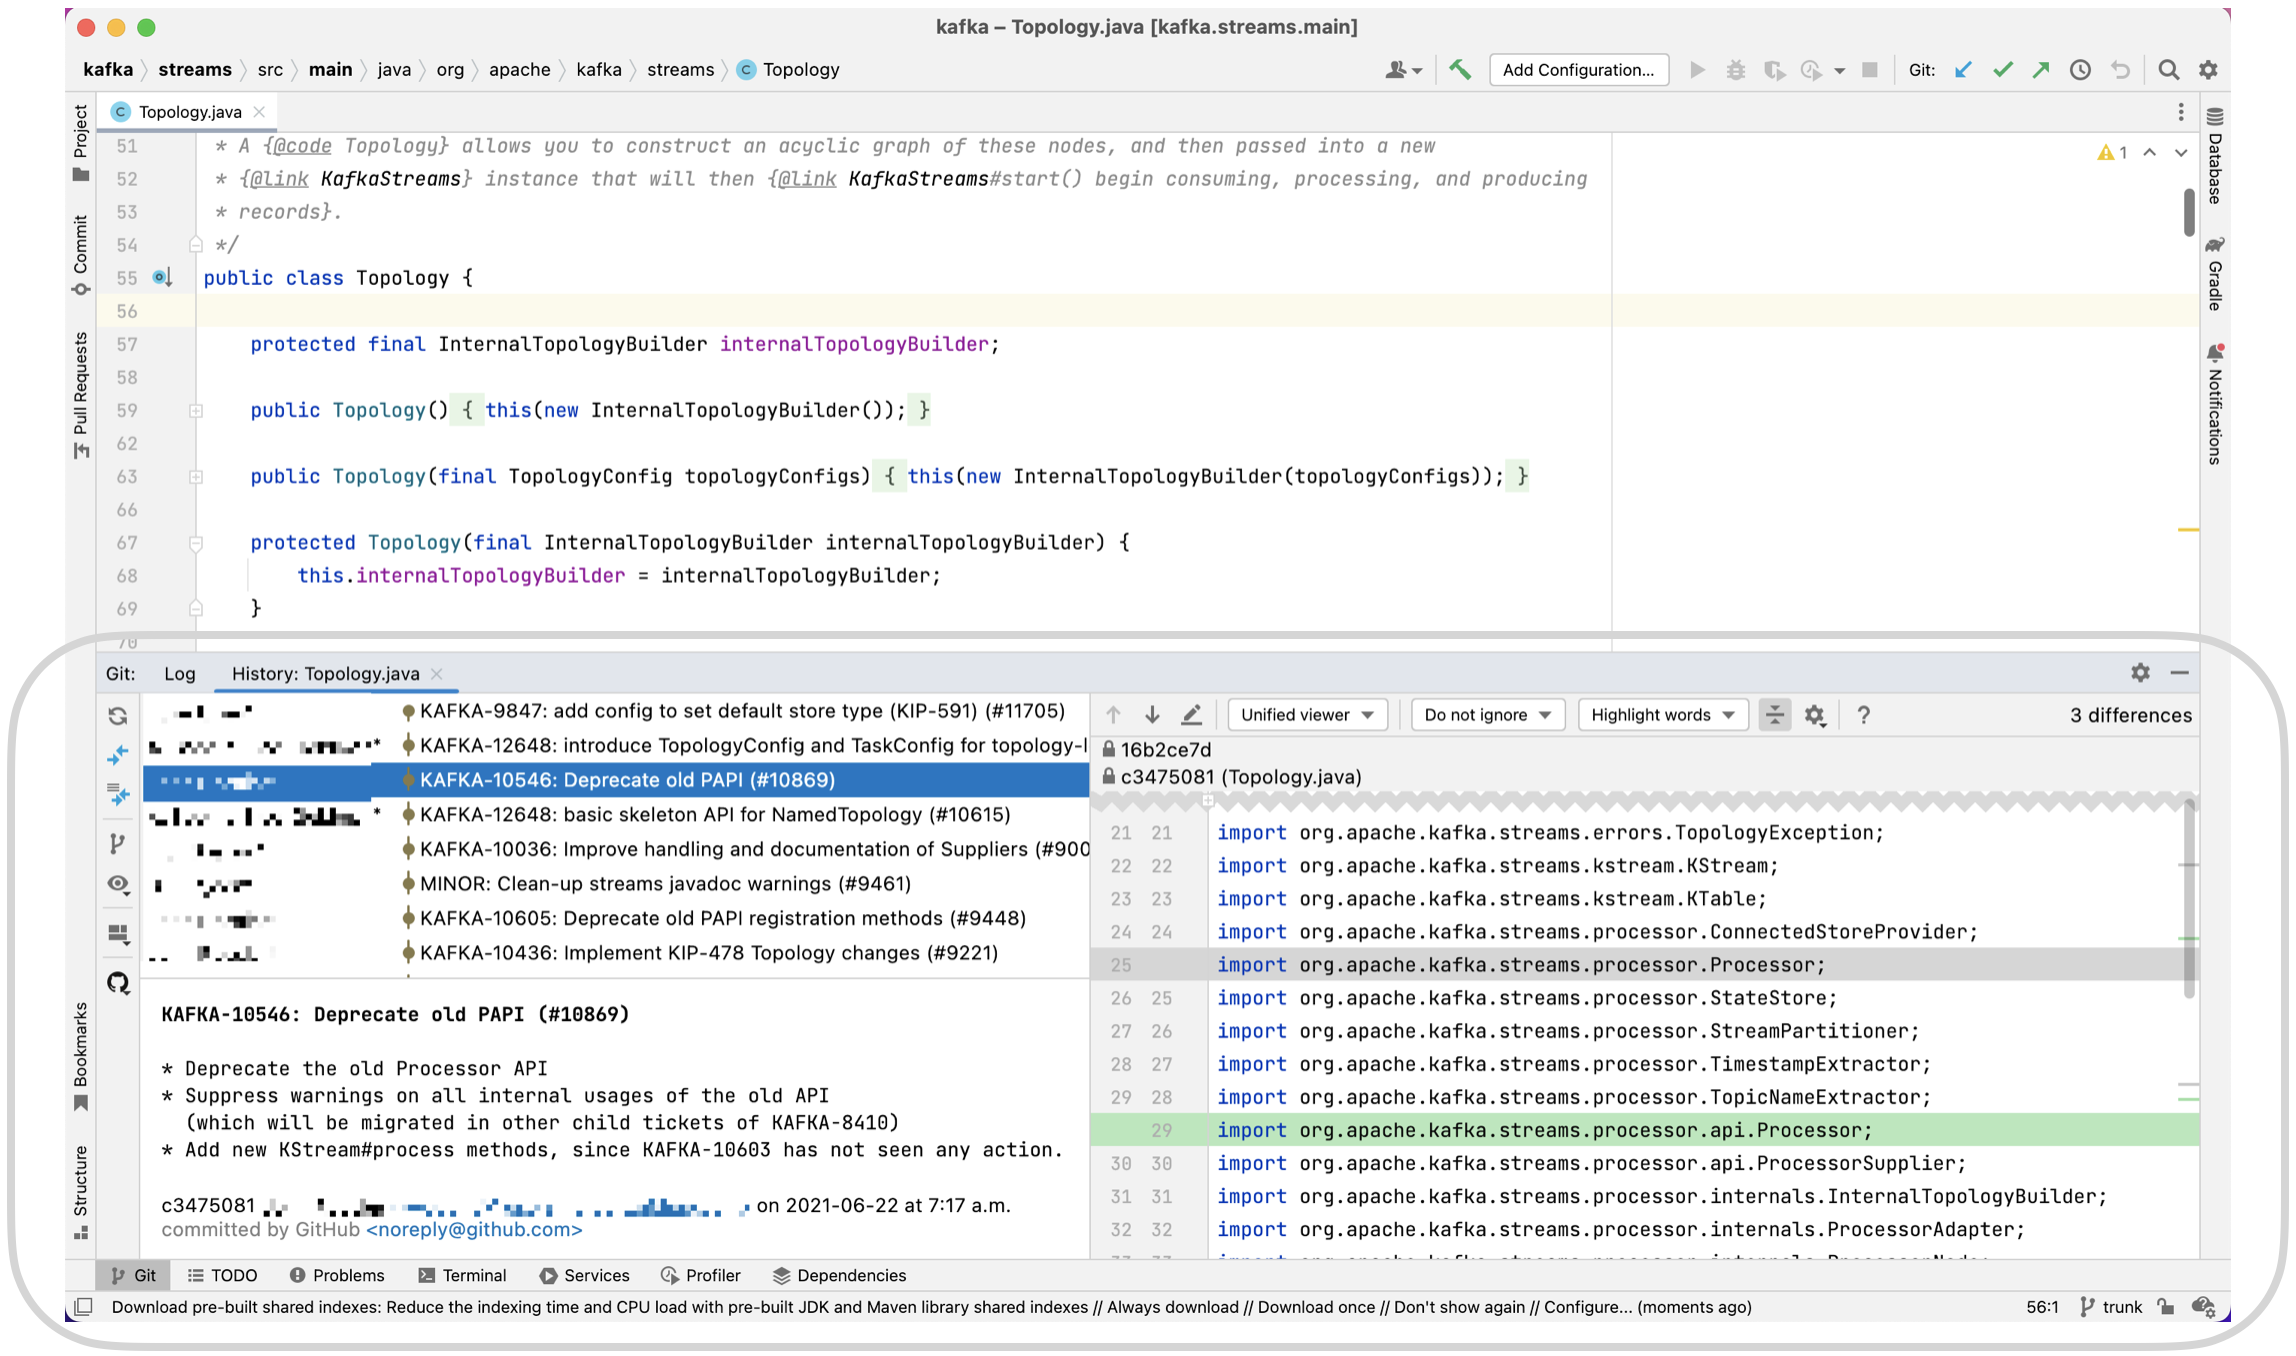
\includegraphics[width=\textwidth]{./images/intellij-overview.png}
    \caption{
        IntelliJ IDEA overview with the built-in Git client displayed on the bottom half. Shows the commit history for the \class{Topology} class in Apache Kafka.
    }
    \label{fig:IntelliJ-Overview}
\end{figure}

\begin{figure}
    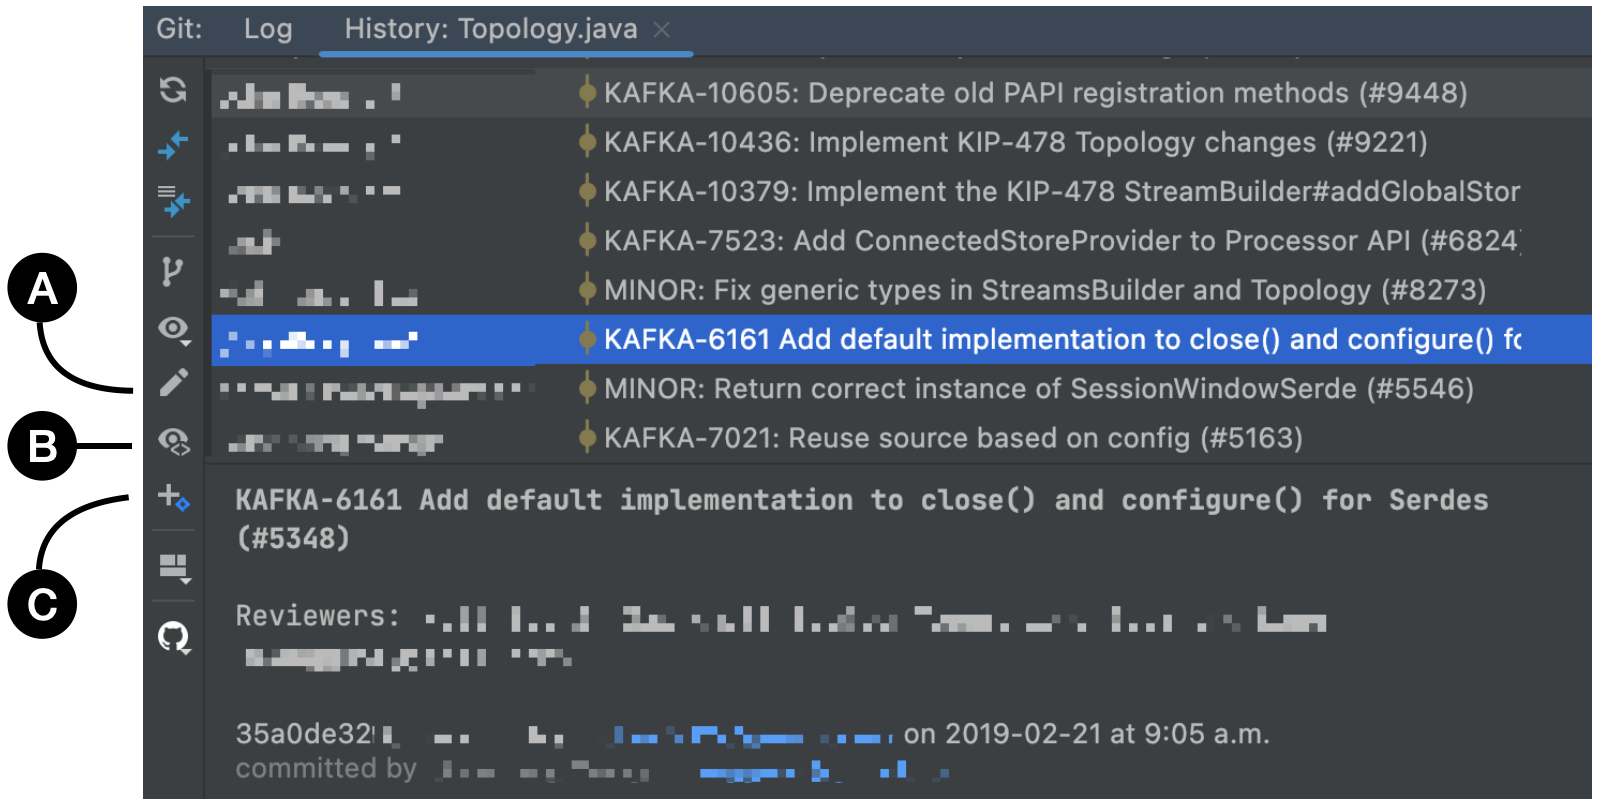
\includegraphics[width=\textwidth]{./images/intelligent-history-overview.png}
    \caption{
        Overview of the actions added by the Intelligent History plugin. We use the following labels: (A) indicates \textit{Highlight Important Changes}; (B) denotes \textit{Show Diff Metadata}; and (C) marks \textit{Show Jira Issue}.
    }
    \label{fig:Intelligent-History-Overview}
\end{figure}

%%%%%%%%%%%%%%%%%%%%%%%%%%%%%%%%%%%%%%%%%%%%%%%%%%%%%%%%%%%%%%%%%%%%%%
\section{Heuristics}
\label{sec:Heuristics}

For distinguishing potentially important commits from less important or trivial commits, we employ a heuristics-based approach to categorize the lines of change in a commit's diff content.
When referring to a commit's diff content, we mean the diff between the old version of a Java class in one commit, and the new version of the Java class after a commit has modified it.
This approach involves scanning the lines between commits for matches to a set of Java code patterns, which describe categories of trivial code changes.
Each pattern is expressed by a form of regular expressions.

While using regular expressions sacrifices some degree of accuracy on what is considered a ``trivial'' line of code change to a user,
regular expressions have the advantage of being lightweight in efficiency and interpretability over other approaches to detecting code changes in programs such as abstract syntax tree (\entity{AST}) matching and differencing techniques \cite{murphy_lightweight_1996}.
Though the advantage of \entity{AST}-level granularity is that it produces edit scripts that directly refer to the structure of code, \entity{AST} matching and differencing techniques having negative performance on runtime and memory consumption, which discouraged us from using them \cite{fluri_change_2007,pawlik_RTED_2011,falleri_fine-grained_2014}.
The goal of our approach is to understand if a minimal set of patterns for expressing trivial code changes can be effective at supporting a software developer in more efficiently navigating software history when searching for code rationale information.

Represented as regular expressions for the Java programming language, our approach for detecting trivial commits uses the following categories for a line of code that has been changed and expressed in a diff: 

\begin{itemize}
    \item \textit{Documentation}: Changes that insert, delete, or modify lines representing single-line or multi-line comments.
    \item \textit{Annotation}: Changes that modify lines representing \code{@Deprecated} annotations or annotations prefixed with \code{@Suppress}.
    \item \textit{Import}: Changes which involve the insertion, deletion, or modification of \code{import} statements.
    \item \textit{Newline}: Changes involving the insertion or deletion of newlines.
    \item \textit{Other}: Any change not classified by the above categories. If a commit has a diff containing at least one change that is not classified by any of the above categories, then the commit is regarded as potentially interesting. Else, a commit is considered less interesting and will be presented as a greyed out commit when the user invokes the \emph{Highlight Import Changes} action.
\end{itemize}

We use the \entity{java-diff-utils} \cite{java-diff-utils} library to extract the diff between two states of a file in the form of deltas. 
To obtain the state of a file for a given commit, we use the IntelliJ Platform's \entity{git4idea} library to retrieve the commits displayed in a file's commit history and the content of the file at the given commit.
The \entity{java-diff-utils} library provides a method that takes an old version $A$ and a new version $B$ of the contents of a file, represented as strings, and produces a list of \emph{abstract deltas} representing each change found from version $A$ to version $B$. 
Each delta contains a list of \emph{source lines} as strings and a list of \emph{target lines} as strings, where source lines represent consecutive lines in version $A$ and target lines represent consecutive lines in version $B$. 
For a set of consecutive lines that have changed from version $A$ to version $B$, a delta would contain the previous state of the lines in source lines and the new state of the lines in target lines.
For a delta that represents an insertion, the source lines would be empty, while the target lines would contain a list of the lines inserted in version $B$.
For a delta that represents a deletion, the target lines would be empty, while the source lines would contain a list of the lines deleted in version $B$.

For each commit in a file's commit history, beginning from the oldest commit to the most recent commit, we obtain the set of deltas for each sequential pair of commits.
Suppose we have a file $F$ and an ordered set of commits representing its commit history as $\{C_{1}, C_{2}, C_{3}, \dots, C_{n}\}$, where $C_{i}$ is a commit that affects $F$ and $i = 1, 2, 3, \dots, n$ denotes the oldest commit to the most recent commit in $F$'s commit history.
We use \entity{java-diff-utils} to obtain the diffs for the state of $F$ in the commit pairs $\{\varnothing, C_{1}\}$, $\{C_{1}, C_{2}\}$, $\{C_{2}, C_{3}\}$, \dots, $\{C_{n-1}, C_{n}\}$.
We compare an empty set, representing an empty string, with the state of $F$ in the first commit $C_{1}$ since the first commit in a file presumably introduces the file $F$ and its initial content.
For each pair of commits, we take the contents of file $F$ in each commit and  obtain a list of deltas and apply regular expression pattern matching on each string in a delta's list of source lines and list of target lines to count the number of lines that match a category.

This categorical information for a user-selected commit is exposed as \emph{diff metadata} in a pop-up when the user invokes the \textit{Show Diff Metadata} action provided by Intelligent History.
For example, \dots \FIXME{Add and reference a figure demonstrating the popup content alongside a commit's diff}.
Exposing this metadata to the user allows the user to obtain a summary about the lines changed from one commit to another commit and to also understand how Intelligent History highlights commits in a file's commit history.

Although we formulated a fixed set of patterns specific to Java, \dots \FIXME{Consider moving this to a section on suggestions for future work? Comment on potential for user-defined patterns.}

%%%%%%%%%%%%%%%%%%%%%%%%%%%%%%%%%%%%%%%%%%%%%%%%%%%%%%%%%%%%%%%%%%%%%%
\section{Issue Metadata}
\label{sec:Issue-Metadata}

\FIXME{Elaborate on the metadata provided in the Jira tool window.}

%%%%%%%%%%%%%%%%%%%%%%%%%%%%%%%%%%%%%%%%%%%%%%%%%%%%%%%%%%%%%%%%%%%%%%
\section{Predictions}
\label{sec:Predictions}

With the interface of Intelligent History established in \autoref{fig:Intelligent-History-Overview}, we describe how we anticipate a user might be able to use the actions from Intelligent History. 
In \autoref{sec:Implementation}, we outlined the three actions a user can invoke while examining a file's history using IntelliJ's built-in file revision history view: (A) \textit{Highlight Important Changes}; (B) \textit{Show Diff Metadata}; and (C) \textit{Show Jira Issue}.

%%%%%%%%%%%%%%%%%%%%%%%%%%%%%%%%%%%%%%%%%%%%%%%%%%%%%%%%%%%%%%%%%%%%%%
\endinput

Any text after an \endinput is ignored.
You could put scraps here or things in progress.
\chapter{User Study}
\label{ch:Evaluation}

To evaluate our hypothesis and the performance of Intelligent History, 
we conducted a user study to observe software developers as they answer questions
requiring them to explore commit histories and obtain code rationale information 
about two Java classes from the Apache Kafka project.
Participants answered a set of questions without Intelligent History,
followed by a different second set of questions with Intelligent History.
We divided up the participants such that we would be able to gather for
two sets of questions that would be answered by participants with and without Intelligent History.
We then followed the observational study of each participant with a semi-structured interview
to gather insight on the participants' experiences with examining commits and issues
and their impressions of Intelligent History.
We targeted the following research questions:

\begin{itemize}[leftmargin=*]
    \item[] \RQ{1}{Can we automatically identify the commits that software developers want to examine?} 
    The underlying approach to commit highlighting involved the construction of regular expression patterns 
    as a minimal set of rules for distinguishing commits containing non-essential changes.
    We ask this RQ to assess the performance of the underlying approach 
    used in Intelligent History's commit highlighting feature (\feature{1}) \textit{Highlight Important Changes}.

    \item[] \RQ{2}{Does highlighting important commits help software developers explore a file’s revision history more efficiently?}
    Our approach to reducing the cognitive burden of examining the commits in a commit history uses commit highlighting in
    the commit history to visually distinguish non-essential commits from potentially more meaningful commits. 
    We propose this RQ to evaluate the contexts in which commit highlighting can help software developers
    investigate a commit history more efficiently, which can be affected by the types of 
    questions software developers seek to answer and the individual approaches and backgrounds of software developers towards
    exploring commit history.

    \item[] \RQ{3}{How useful is direct integration of issue information in the IDE for helping a developer search for code rationale information?}
    In our implementation of feature (\feature{3}) \textit{Show Jira Metadata}, we integrated a view of a Jira issue's title, description, reporter, assignee, priority,
    and metadata information related to the number of comments and linked issues to give the plugin user a signal 
    of how interesting a Jira issue might be for further examination.
    This RQ seeks to gauge how useful is presenting issue information in the same context as the commit history and source for a file.
\end{itemize}

We describe the method we designed to address these research questions in detail in \autoref{sec:Method}.
We present the results of our analysis and answer the research questions in \autoref{sec:Results}.

%%%%%%%%%%%%%%%%%%%%%%%%%%%%%%%%%%%%%%%%%%%%%%%%%%%%%%%%%%%%%%%%%%%%%%
\section{Method}
\label{sec:Method}

We designed the user study to consist of two parts,
an observational study and a semi-structured interview, 
with an estimated combined duration of 1 to 1.5 hours.
For the first part, the observational study allows us to obtain a real-time 
portrayal of how the participants explore and interact with commit history,
and how the presence of Intelligent History influences the participants'
examination of commits to obtain answers to code rationale questions \cite{shull_guide_2007}.
For the second part, the semi-structured interview format allows us to maintain a focused discussion 
while also eliciting interesting responses and reasoning from participants \cite{shull_guide_2007}.
The briefing for the study and the setup instructions can be found in Appendix \ref{sec:Briefing-and-Setup}.
We expected the participants to interact with commit and issue information 
found in the commit history in order to be able to answer these questions.

\subsection{Observational Study}

The observational study involved having participants explore the commit history of two Java classes 
from the Apache Kafka project in the IntelliJ IDEA \entity{IDE} 
to find answers to questions related to motivation and rationale behind changes in the classes.
Apache Kafka is an event streaming platform used to collect, process, and store streaming event data.
We chose to use Apache Kafka because the project's contribution guidelines mandates that
each commit's message must be prefixed with a Jira issue ID, of the form \issue{KAFKA-XXXX},
excluding minor commits prefixed with \issue{MINOR} or hotfixes prefixed with \issue{HOTFIX}.
This convention in Apache Kafka will allow the user to exercise all of the features of Intelligent History
as meaningful commits will generally be associated with a Jira issue in the Apache Kafka project.

Moreover, Apache Kafka also has a practice of maintaing Kafka Improvement Proposals (\entity{KIP}s),
which are documents intended to capture the thought process behind major features introduced 
and changes that impact the public Kafka \entity{API}s.
Commits in the Apache Kafka repository that include changes that are part of \entity{KIP}s will
reference them in their commit messages.
\entity{KIP}s typically have a section titled ``Motivation,''
which can help participants since our observational study will use the commit history 
in Apache Kafka will involve asking the participants to find code rationale information.

The observational part of the user study session consists of 
asking the participants questions about two Java classes from Apache Kafka.
The questions are presented as A1, A2, B1, and B2 in \autoref{tab:Question-Sets}.
Questions A1 and A2 are from set A, while questions B1 and B2 are from set B.
Set A asks about the \class{Topology} class from Apache Kafka and 
set B asks about the \class{StreamsBuilder} class from Apache Kafka.
The \class{Topology} class for set A contains 22 commits and the \class{StreamsBuilder} class for set B contains 45 commits.
The questions are not timed and participants we allow participants to explore the commit history and read Jira issues at their own pace.
We limit the number of questions to two questions per class based on the number of commits in each class' commit history and 
to accomodate keeping the estimated duration of the study as a laboratory experiment within a reasonable amount of time.

All questions require the participant to explore and locate particular commits or changes 
from a Java class' commit history to try to find code rationale information that can
help them formulate an answer to each question.
For each question, we expect the participant to inspect a commit's full message,
diffs, and any relevant Jira issues to be able to answer the questions.
For example, to answer A2, participants must find a commit that introduced further \code{addSink} method overloads 
later in the commit history to be able to find the intent behind the decision.
The commit which does this is \commitref{f33e9a34}{https://github.com/apache/kafka/commit/f33e9a346e22e29bb66e0ea0f3442903d136ca67} 
and has the following commit message title:

\begin{center}
  \jira{KAFKA-4936:}{Add dynamic routing in Streams (\#5018)} 
\end{center}

Participants are not expected to be able to identify this commit based on the commit message title alone.
However, participants will be informed that the first commit in the \class{Topology} class introduced a series of \code{addSink} overloads already.
Participants then might strategize by examining the diffs of commits
that were made after the first commit in the \class{StreamsBuilder} commit history 
that introduced an initial set of overloaded \code{addSink} methods.
To find the intent behind this addition of methods,
the participant would need to read the referenced Jira issue \issue{KAFKA-4936}.
In cases where a Jira issue references a Kafka Improvement Proposal (\entity{KIP}), 
we allow the participant to visit these \entity{KIP}s in the browser.

\begin{table}[h]
  \caption{
    The question sets used in the user study. 
    Set A pertains to the \class{Topology} class (22 commits) and set B relates to the \class{StreamsBuilder} class (45 commits).
  }
  \centering
  \footnotesize
  \begin{tabular}{@{}c|c|ll@{}}
    \toprule
    Class                           & Set                & \multicolumn{2}{c}{Question}                                                                                                                                                                                                                                                                                                                                      \\ \midrule
    \multirow{2}{*}{\class{Topology}}       & \multirow{2}{*}{A} & \multicolumn{1}{l|}{A1} & \begin{tabular}[c]{@{}l@{}}Can you describe the motivation behind why the\\ code segment on lines 717 to 722 was introduced and the\\ benefit to the user of the Kafka \entity{API}?\end{tabular}                                                                                                                                                \\ \cmidrule(l){3-4} 
                                    &                    & \multicolumn{1}{l|}{A2} & \begin{tabular}[c]{@{}l@{}}There are several overloaded methods called \code{addSink} \\ in this class. \\ Can you describe in what context\\ were these overloaded methods introduced to this class?\end{tabular}                                                                                                                             \\ \midrule
    \multirow{2}{*}{\class{StreamsBuilder}} & \multirow{2}{*}{B} & \multicolumn{1}{l|}{B1} & \begin{tabular}[c]{@{}l@{}}Can you find two commits that introduced changes to\\ improve some functionality in this class and justify why\\ you chose them? \\ The changes can not be cosmetic such as removing \\ repeated words, removing deprecated code,\\ or adding/modifying/removing documentation \\ and comments.\end{tabular} \\ \cmidrule(l){3-4} 
                                    &                    & \multicolumn{1}{l|}{B2} & \begin{tabular}[c]{@{}l@{}}Why is the build method in this class overloaded?\\ Specifically, why was the overloaded \code{build} method in\\ lines 623 to 630 introduced?\end{tabular}                                                                                                                                                         \\ \bottomrule
  \end{tabular}
  \label{tab:Question-Sets}
\end{table}

We created two different sets, A and B, to facilitate our observation
of how a participant investigates the commit history without Intelligent History
for the first set of questions and with Intelligent History for the second set of questions.
After completing the first provided set of questions, 
the participant is introduced to the features of the Intelligent History plugin 
and may use them to help them find the information needed to answer 
the second set of questions they receive.

We divide the participants into two groups such that one group received 
and completed question set A first without using the Intelligent History plugin 
and question set B afterwards with introduction to the plugin and its features.
The other group received set B first to complete without the plugin
and set A to complete with the plugin.
We swapped the order of the sets for the groups 
to observe and collect data about the performance of Intelligent History for each set.

To assess the quality and correctness of a participant's answer, 
we prepared an answer key, which is available in \autoref{tab:Answer-Key}.
For questions A1, A2, and B2, there were specific commits we identified as answers.
For B1, we anticipated a range of possible answers that a participant could provide.
The criteria for sufficient completion of a question was based on the participant's ability 
to provide a justification to their answer through referencing relevant parts of the source code, commit messages, Jira issues, and
identification of a commit author's intent or the motivation behind a change.

The participants provided their answer to each question verbally to the author of this thesis, 
who served as an observer and interviewer for each participant's user study session.
We permit participants to think aloud.
Prior to commencing the study, we also inform the participants we encourage them to discuss their approach 
as to how plan to find the information they need to answer the questions they are provided.
The observer refrained from guiding the participant to an answer to avoid 
giving the participant any expectation to use any particular strategy.
However, if a participant expressed struggling or confusion on how to obtain the 
information needed to answer a question, the observer would remind the participant about
about the sources of information at their disposal or prompt the participant to verbalize
their confusion or approaches to a question.

\begin{landscape}
  \begin{table}[]
      \caption{Answer key for the questions presented in \autoref{tab:Question-Sets}.}
      \centering
      \footnotesize
      \begin{tabular}{@{}c|l@{}}
      \toprule
      Question & \multicolumn{1}{c}{Answer}                                                                                                                                                                                                                                                                                                                                                                                                                                                                                                                                                                                                                              \\ \midrule
      A1       & \begin{tabular}[c]{@{}l@{}}The participant should find commit \commit{075bbcfe} and reference the Jira issue \fnissue{KAFKA-7523}.\\ The change implicitly connects state stores to processors/transformers to avoid burdening the API user\\ with having to explicitly specify the stores.\end{tabular}                                                                                                                                                                                                                                                                                                                                                                   \\ \midrule
      A2       & \begin{tabular}[c]{@{}l@{}}The participant should find commit \commit{f33e9a34} and reference the Jira issue \fnissue{KAFKA-4936}.\\ The participant is expected to deliver a summary referencing the following motivation behind the change: \\ Allow users to dynamically choose which topic to send to at runtime, which can help remove the burden of \\ having to update and restart KStreams applications. \end{tabular}                                                                                                                                                        \\ \midrule
      B1       & \begin{tabular}[c]{@{}l@{}}Possible answers:\\ \commit{075b368d} (\fnissue{KAFKA-6958}) allows the user to define custom names for processors with the KStreams DSL to make \\ complex topologies easier to understand.\\ \commit{3e64e5b9} (\fnissue{KAFKA-6761}) reduces the footprint of Kafka Streams, which reduces resource utilization. \\ \commit{c0353d8d} (\fnissue{KAFKA-6036}) optimizes when to use logical materialization, related to reducing the Kafka Streams footprint. \\ The participant should choose commits which improve some functionality in the \class{StreamsBuilder} class\\ and justify their answer by understanding commit author intent.\\ If the commit intends to fix a bug, the participant should describe the bug and how the commit resolved the bug.\\ The participant may not choose commits which only modify comments, fix typos, add newlines.\end{tabular} \\ \midrule
      B2       & \begin{tabular}[c]{@{}l@{}}The participant should find commit \commit{e09d6d79} and reference the Jira issue \fnissue{KAFKA-7027}.\\ The overloaded \code{build} method provides the option to accept user-defined configurations which have the required values for \\ building the Kafka topology.\\ This controls optimization by leaving the construction of the topology to the overloaded build \code{method}.\end{tabular}                                                                                                                                                                                                                                                        \\ \bottomrule
      \end{tabular}
      \label{tab:Answer-Key}
  \end{table}
\end{landscape}

\subsection{Interview}

The second part of the session consisted of asking a series of open-ended interview questions to gather information about 
the participant's background with respect to software development and experience in examining commits and issues from an issue tracking system.
We also asked participants to compare their experience in completing the question sets without and with the use of Intelligent History.
The interview questions are available in \autoref{fig:Interview-Questions}.
As part of the semi-structured interview format, 
we anticipate asking follow-up questions based on the participant's responses for further clarification 
and to probe further about unexpected responses \cite{shull_guide_2007}. 

\begin{figure}[h]
  \begin{mdframed}
    \footnotesize
    \begin{enumerate}
      \item How many years of software development experience do you have, both professionally and non-professionally?
      \item In your development experience, have you often looked at commits and the issues associated with them (e.g. GitHub issues/pull requests, Jira issues, Bugzilla, etc.)?
          \begin{enumerate}
              \item In what scenarios or kinds of tasks do you typically look at commits and issues?
              \item How would you usually go about obtaining answers to questions about the intent behind the code you are reading?
          \end{enumerate}
      \item What types of code changes or content in diffs do you think are less useful or more useful when trying to understand why a developer wrote code a certain way or made a particular change? 
          \begin{enumerate}
              \item What changes in diffs do you think make a commit more important or less important to look at?
          \end{enumerate}
      \item For the task involving use of the plugin, which features did you find helpful/unhelpful to your exploration?
      \item Are there any comments or feedback you would like to provide?
    \end{enumerate}
\end{mdframed}
  \caption{The interview questions asked in the semi-structured interview part of the user study.}
  \label{fig:Interview-Questions}
\end{figure}

The user study sessions took place virtually over Zoom, where participants were asked to share their screen.
We recorded all of the sessions and used the recordings to document each session with a summary.

\subsection{Participants}

We recruited 10 participants through public posting on social media and circulating a letter of initial contact within the author's professional network.
We focused on recruiting software developers with at least 1 year of experience in software development, 
which could include non-professional and professional experience.
Participants were compensated with entrance to a raffle for 1 of 5 Amazon gift cards valued at $\$40$ \entity{CAD}.
\autoref{tab:Participants} shows the demographic information we collected for each participant and 
which question set, from A and B, that the participant received first and second.
The participant is always introduced to the features of the Intelligent History plugin after completing the first of questions and 
is permitted to use the plugin features for the second set of questions.
The role for each participant indicates their occupation title at the time of the user study.
We generalized the participants' roles to uphold their anonymity.
Among the 10 participants, 4 were students and 6 were professional developers.
In terms of the participants' total years of experience in software development, 
the mean was 5.2 years and the median was 4.3 years.

\begin{table}[h]
  \caption{
    Participants by pseudo-initial, total years of experience (YoE) with separation 
    by professional (p) and non-professional (n-p) experience, current role, and 
    the question set the participant received first and second.
  }
  \centering
  \begin{tabular}{@{}c|clcc@{}}
  \toprule
  \multicolumn{1}{l}{Pseudo-initial} & \multicolumn{1}{l}{YoE (p/n-p)} & \multicolumn{1}{c}{Role} & \multicolumn{1}{l}{First Set} & \multicolumn{1}{l}{Second Set} \\ \midrule
  A                                  & 4.0 (1.0/3.0)                   & Firmware Developer       & A                             & B                               \\
  B                                  & 3.0 (2.8/0.2)                   & Software Developer       & B                             & A                               \\
  C                                  & 6.0 (3.0/3.0)                   & UX Engineer              & A                             & B                               \\
  D                                  & 4.5 (2.5/2.0)                   & Software Developer       & B                             & A                               \\
  E                                  & 13.0 (6.0/7.0)                  & Graduate Student         & A                             & B                               \\
  F                                  & 6.0 (2.0/4.0)                   & Software Developer       & B                             & A                               \\
  G                                  & 2.0 (0.0/2.0)                   & Undergraduate Student    & A                             & B                               \\
  H                                  & 3.5 (1.5/2.0)                   & Software Developer       & B                             & A                               \\
  I                                  & 4.0 (3.0/1.0)                   & Graduate Student         & A                             & B                               \\
  J                                  & 6.0 (2.0/4.0)                   & Graduate Student         & B                             & A                               \\ \bottomrule
  \end{tabular}
  \label{tab:Participants}
\end{table}

\subsection{Analysis}

\subsubsection{Quantitative Analysis}

To support quantitative analysis of Intelligent History, 
we instrumented the Intelligent History plugin to log timestamps and events occuring within the IDE
for both the first and second sets of questions that a participant answered.
Although we asked participants to install the Intelligent History plugin prior to commencing the
observational study, we did not introduce the participant to the features of Intelligent History 
or permit the participant to use any features from the plugin until completion of the first set of questions.
For the events, we logged the commits that a participant examined for each question 
and the actions of Intelligent History that the participant invoked,
including the toggling of (\feature{1}) \textit{Highlight Important Changes} 
and the invocation of both (\feature{2}) \textit{Show Diff Metadata} and (\feature{3}) \textit{Show Jira Metadata}.
This enables us to record the number of commits that a participant investigated to answer a question 
and how the participant interacted with the Intelligent History plugin for answering the question set in which they were permitted to use its features.
We can also trace which specific commits a participant examined as part of their search and if a commit was 
or would have been highlighted by Intelligent History.
From the quantitative metrics, we record the number of commits from a file's commit history that a participant examined 
and skimmed to answer each question as a percentage of the number of commits from the file's commit history.
We define skimming as when a participant read's a commit message's title aloud, but does not select the commit in the commit history
for further inspection of the diff or the full commit message.

For each question that a participant answers, we also record the proportion of a participant's examined commits 
that are highlighted commits according to Intelligent History,
the number of application switches a user makes between the \entity{IDE} and their browser for viewing Jira issues,
and the number of Jira issues that a participant viewed or accessed.
For the question set in which the participant was permitted to use Intelligent History, 
we consider the invocation of (\feature{3}) as viewing a Jira issue since the content of the issue is accessed from within the \entity{IDE}.

After obtaining the quantitative data, we conduct a single-tailed, two-sample $t$-test to test for statistically significant differences 
between the proportion of commits examined by the group of participants that completed a question without Intelligent History and the group of participants 
that completed the same question with Intelligent History.
We use the following null hypothesis ($H_{0}$) for each question asked in the user study: 
\textit{The mean proportion of commits from a commit history examined by the group without Intelligent History and the group with Intelligent History are equal.}
For each question asked in the user study, we compute the $t$-value and $p$-value for the group that completed 
the question without Intelligent History and the group that completed the question with Intelligent History.
For the significance level $\alpha = 0.05$, we reject the null hypothesis if $p < 0.05$.
Each group contains 5 samples, hence the degrees of freedom for each $t$-test is $df = 8$.

\subsubsection{Qualitative Analysis}

To support qualitative analysis, we used the session recordings and collected plugin logs to construct directed graphs 
for each participant's session to visualize how they explored commit history to answer the question sets 
and the impact of Intelligent History on their exploration.
We regard these graphs as \emph{commit history exploration graphs} and constructed a set of these graphs for each participant, 
one for each question the participant worked on.
We provide a sample of two commit history exploration graphs we constructed to illustrate 
participants \participant{F} and \participant{H}’s exploration to answer question B1 
from \autoref{tab:Question-Sets} in \autoref{fig:Exploration-Graphs}.
For B1, both participant \participant{F} and \participant{H} did not use Intelligent History.
Nodes in the graph are represented by commit hashes and Jira issue IDs, 
while edges express the participant's movement from examining one commit to another.
Bold commit hashes denote commits that would be highlighted by Intelligent History, 
while light hashes indicate non-highlighted commits.
Italicized commit hashes are those for which the participant was heard reading or skimming the commit message subject aloud, 
but did not investigate further by explicitly selecting the commit for further viewing.
We use a green checkmark to signal when a participant provided a sufficient answer to the question 
and a globe icon to show when a participant made an application switch between the \entity{IDE} 
and their browser to further examine a Jira issue.

\begin{figure}[h]
  \centering%
  \subfloat[\centering \participant{B}'s commit history exploration in answering question B1 without Intelligent History. \label{subfig:Exploration-Graph-A}]{{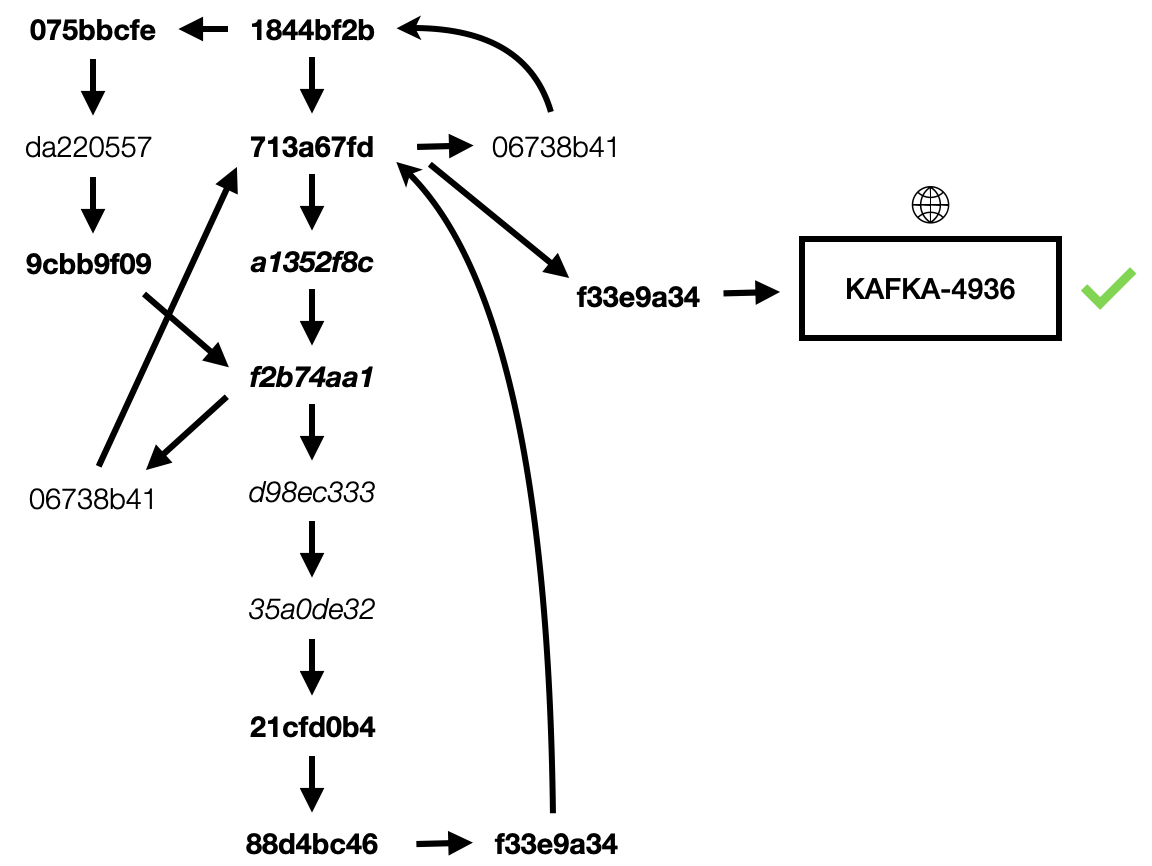
\includegraphics[width=5.5cm]{./images/graph-sample-A.png}}}%
  \qquad
  \subfloat[\centering \participant{H}'s commit history exploration in answering question B1 without Intelligent History. \label{subfig:Exploration-Graph-B}]{{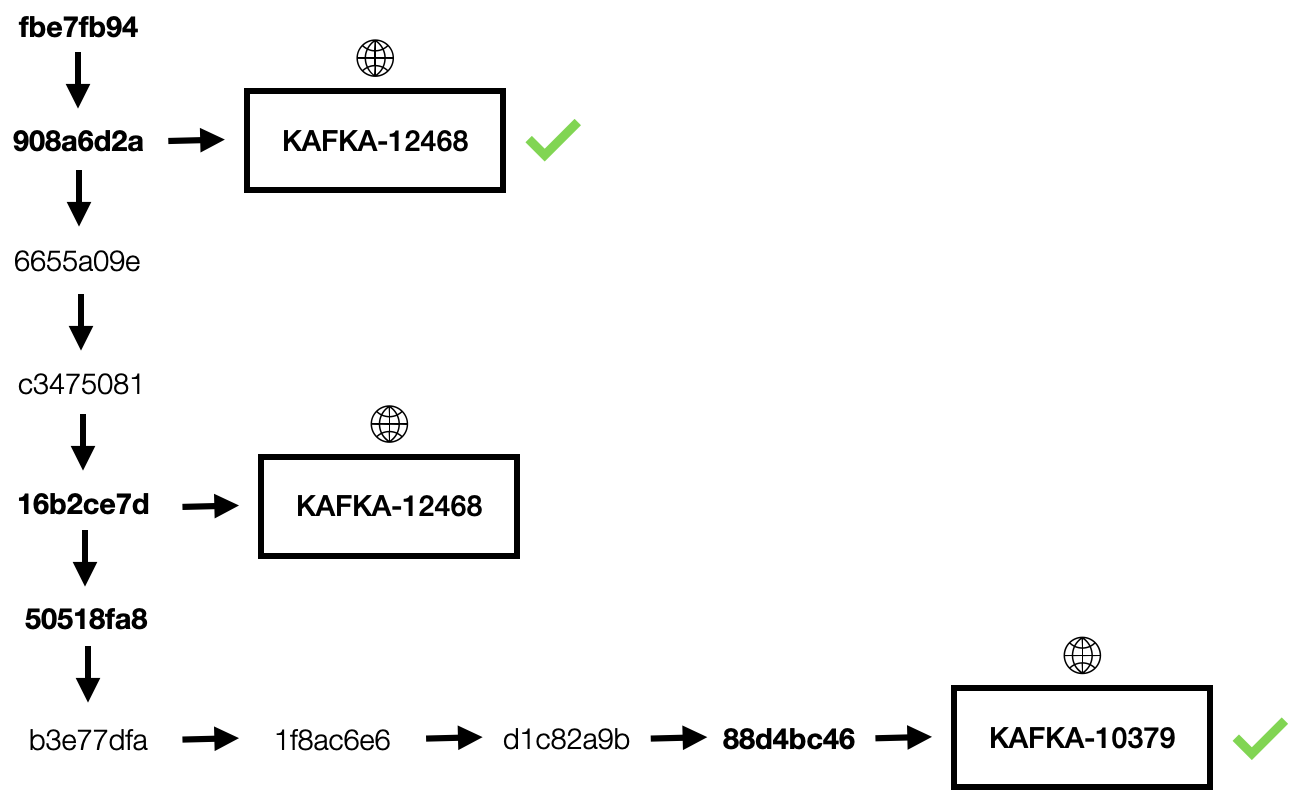
\includegraphics[width=5.5cm]{./images/graph-sample-B.png}}}%
  \caption{
    Commit history exploration graphs.
  }%
  \label{fig:Exploration-Graphs}%
\end{figure}

We determine a participant's commit history exploration approach based on the structure 
of the participant's commit history exploration graphs and from reviewing the user study session recordings.
A participant's exploration approach is categorized as one of:
\textit{linear}, \textit{cyclic and backtracking}, or \textit{commit message skimming}.
We define \textit{linear} for directed graphs in which all of the nodes represent commits 
that were examined in chronological order by timestamp. 
We use \textit{cyclic and backtracking} to describe directed graphs 
containing more than three cycles, indicating that the participant has backtracked to
an earlier seen commit at least three times, causing a cycle. 
Lastly, \textit{commit message skimming} characterizes graphs where 
at least half of the nodes are italicized commit hashes to indicate
that the commit messages were only glanced at by the participant but the
contents of the commit were not further inspected by the participant.
If the condition for a graph to be categorized as \textit{commit message skimming} is met,
we categorize the graph as such regardless of whether the graph meets the critiera for the other two categories.

For each participant, we use the commit history exploration graph for question B1
as a starting point to characterize the participant's exploration approach since
B1 requires interaction with the larger commit history of the two files the participants were asked to explore.
B1 is also only answerable by considering several commits in the commit history since the
participant must make sure that the commits they select to use in their answer meet the conditions specified in the question.
For cases where a participant's graph for B1 may fit into more than one category for a commit history exploration approach,
we used the participant's graphs for A1, A2, and B2 to determine the dominant structure we observed across all graphs.

As a demonstration of how we devised categories for the participants' exhibited approaches for commit history exploration, 
\autoref{subfig:Exploration-Graph-A} illustrates participant \participant{B}'s approach to finding 
two meaningful commits as per question B1 without using Intelligent History.
The commit history exploration graph for \participant{B} shows they examined 16 out of 45 commits.
Participant \participant{B} would examine a few commits at a time,
as seen by the long linear series of commits explored in the left side of \autoref{subfig:Exploration-Graph-A}.
Participant \participant{B} then backtracked to previously seen commits 
after gaining a broad sense of the changes made over time to the file,
as seen by the jumps between \commit{059a81e3} back to the beginning of their search at \commit{fbe7fb94}, 
then to later to \commit{88d4bc46} and back to \commit{908a6d2a}.
We characterize the structure of the graph for \participant{B} as \textit{cyclic and backtracking},
given the three cycles in the graph we observed.

Meanwhile, the commit history graph for \participant{H} shown in \autoref{subfig:Exploration-Graph-B}, 
who answered the same question without Intelligent History, shows they examined 10 out of 45 commits.
Participant \participant{H} systematically examined 
each commit sequentially in chronological order by each commit's timestamp.
We characterize the structure of the graph for \participant{H} and their commit history exploration approach as \textit{linear} 
to describe the participant's sequential exploration of the commit history.

To analyze the participants' responses to the open-ended, semi-structured interview questions, 
we create a flowchart to illustrate the relationship between each participant's experience with looking at issues and commits,
the commit history exploration approach they exhibitied when searching for the answers to the question sets, 
and the features of Intelligent History for which they expressed the most enthusiasm.
In the interviews, we asked participants how often they looked at commits and issues 
and categorized their responses as: 
\textit{often}, \textit{sometimes}, or \textit{rarely}.
We determined the feature of Intelligent History that a particiant found most favourable from
(\feature{1}) \textit{Highlight Important Changes}, 
(\feature{2}) \textit{Show Diff Metadata}, and
(\feature{3}) \textit{Show Jira Metadata}
based on a trend we observed in the participants' responses to interview question (4) from \autoref{fig:Interview-Questions}.
When interviewed about comparing their experience with and without using Intelligent History,
participants typically stated the feature of Intelligent History to which they responded most positively.

%%%%%%%%%%%%%%%%%%%%%%%%%%%%%%%%%%%%%%%%%%%%%%%%%%%%%%%%%%%%%%%%%%%%%%
\section{Results}
\label{sec:Results}

%%%%%%%%%%%%%%%%%%%%%%%%%%%%%%%%%%%%%%%%%%%%%%%%%%%%%%%%%%%%%%%%%%%%%%

\subsection{RQ1}
\label{subsec:RQ1}

\RQ{1}{Can we automatically identify the commits that software developers want to examine?}

We summarize the quantitative results collected through logs and screen recordings in \autoref{tab:Results-Quantitative-AB} 
for participants who received question set A first, then set B.
Likewise, the results for participants who received question set B first, then set A are summarized in \autoref{tab:Results-Quantitative-BA}.
As stated in \autoref{sec:Method}, question set A corresponds to the \class{Topology} class, which contains 22 commits in its commit history, 
while set B corresponds to the \class{StreamsBuilder} class, which contains 45 commits in its commit history.
Overall, participants who did not use Intelligent History examined a higher mean proportion of commits for questions A1, A2, and B1.

%% BEGIN: Large landscape tables
\begin{landscape}
  \begin{table}
    \footnotesize
    \caption{
      Summary of results for participants who received question set A first to complete without the plugin and question set B after to complete with the plugin.
      For each question set and question, the table shows the percentage of commits from the commit history that the participant examined (\%CE), 
      the percentage of the participant's examined commits that would be or were highlighted by the plugin (\%HC),
      the number of application switches between the \entity{IDE} and the browser (\#AC) that the participant made,
      and the number of Jira issues the participant viewed or accessed (\#IV).
    }
    \centering
    \begin{tabular}{@{}ccccccccccccccccc@{}}
      \toprule
      \multicolumn{1}{l}{}                & \multicolumn{8}{c}{Set A (without plugin)}                                                                                                                            & \multicolumn{8}{c}{Set B (with plugin)}                                                                                                                                                                 \\ \midrule
      \multicolumn{1}{c|}{}               & \multicolumn{4}{c|}{A1}                                  & \multicolumn{4}{c|}{A2}                                                                                    & \multicolumn{4}{c|}{B1}                                                                     & \multicolumn{4}{c}{B2}                                                                                    \\ \midrule
      \multicolumn{1}{c|}{Pseudo-initial} & \%CE      & \%HC      & \#AS & \multicolumn{1}{l|}{\#IV} & \multicolumn{1}{l}{\%CE} & \multicolumn{1}{l}{\%HC} & \multicolumn{1}{l}{\#AS} & \multicolumn{1}{l|}{\#IV} & \%CE      & \multicolumn{1}{l}{\%HC} & \multicolumn{1}{l}{\#AS} & \multicolumn{1}{l|}{\#IV} & \multicolumn{1}{l}{\%CE} & \multicolumn{1}{l}{\%HC} & \multicolumn{1}{l}{\#AS} & \multicolumn{1}{l}{\#IV} \\ \midrule
      \multicolumn{1}{c|}{A}              & 40.9 (9)  & 55.6 (5)  & 1    & \multicolumn{1}{c|}{1}    & 27.3 (6)                 & 83.3 (5)                 & 1                        & \multicolumn{1}{c|}{1}    & 15.6 (7)  & 100.0 (7)                & 0                        & \multicolumn{1}{c|}{4}    & 6.7 (3)                  & 100.0 (3)                & 0                        & 1                        \\
      \multicolumn{1}{c|}{C}              & 4.5 (1)   & 100.0 (1) & 1    & \multicolumn{1}{c|}{1}    & 27.3 (6)                 & 83.3 (5)                 & 1                        & \multicolumn{1}{c|}{1}    & 6.7 (3)   & 100.0 (3)                & 0                        & \multicolumn{1}{c|}{2}    & 0.0 (0)                  & N/A                      & 0                        & 0                        \\
      \multicolumn{1}{c|}{E}              & 36.3 (8)  & 62.5 (5)  & 1    & \multicolumn{1}{c|}{1}    & 68.1 (15)                & 66.7 (10)                & 1                        & \multicolumn{1}{c|}{1}    & 35.6 (16) & 100.0 (16)               & 1                        & \multicolumn{1}{c|}{3}    & 8.9 (4)                  & 100.0 (4)                & 0                        & 1                        \\
      \multicolumn{1}{c|}{G}              & 86.3 (19) & 57.9 (11) & 1    & \multicolumn{1}{c|}{1}    & 36.3 (8)                 & 75.0 (6)                 & 1                        & \multicolumn{1}{c|}{1}    & 13.3 (6)  & 100.0 (6)                & 3                        & \multicolumn{1}{c|}{5}    & 6.7 (3)                  & 100.0 (3)                & 1                        & 2                        \\
      \multicolumn{1}{c|}{I}              & 4.5 (1)   & 83.3 (5)  & 1    & \multicolumn{1}{c|}{1}    & 36.3 (8)                 & 75.0 (6)                 & 1                        & \multicolumn{1}{c|}{1}    & 6.7 (3)   & 100.0 (3)                & 0                        & \multicolumn{1}{c|}{2}    & 6.7 (3)                  & 100.0 (3)                & 0                        & 1                        \\ \midrule
      \multicolumn{1}{l|}{Mean}           & 34.5      & 68.5      & 1    & \multicolumn{1}{c|}{1}    & 39.1                     & 76.7                     & 1                        & \multicolumn{1}{c|}{1}    & 15.6      & 100.0                    & 0.8                      & \multicolumn{1}{c|}{3.2}  & 5.8                      & 100.0                    & 0.2                      & 1                        \\
      \multicolumn{1}{l|}{Median}         & 36.3      & 62.5      & 1    & \multicolumn{1}{c|}{1}    & 36.3                     & 75.0                     & 1                        & \multicolumn{1}{c|}{1}    & 13.3      & 100.0                    & 0.0                      & \multicolumn{1}{c|}{3.0}  & 6.7                      & 100.0                    & 0.0                      & 1                        \\ \bottomrule
    \end{tabular}
    \label{tab:Results-Quantitative-AB}
  \end{table}
\end{landscape}

\begin{landscape}
  \begin{table}
    \footnotesize
    \caption{
      Summary of results for participants who received question set B first to complete without the plugin and question set A after to complete with permitted use of the plugin.
      The same columns as shown in \autoref{tab:Results-Quantitative-AB} are used.
    }
    \centering
    \begin{tabular}{@{}ccccccccccccccccc@{}}
      \toprule
      \multicolumn{1}{l}{}                & \multicolumn{8}{c}{Set A (with plugin)}                                                                                                                              & \multicolumn{8}{c}{Set B (without plugin)}                                                                                                                                                              \\ \midrule
      \multicolumn{1}{c|}{}               & \multicolumn{4}{c|}{A1}                                 & \multicolumn{4}{c|}{A2}                                                                                    & \multicolumn{4}{c|}{B1}                                                                     & \multicolumn{4}{c}{B2}                                                                                    \\ \midrule
      \multicolumn{1}{c|}{Pseudo-initial} & \%CE     & \%HC      & \#AS & \multicolumn{1}{l|}{\#IV} & \multicolumn{1}{l}{\%CE} & \multicolumn{1}{l}{\%HC} & \multicolumn{1}{l}{\#AS} & \multicolumn{1}{l|}{\#IV} & \%CE      & \multicolumn{1}{l}{\%HC} & \multicolumn{1}{l}{\#AS} & \multicolumn{1}{l|}{\#IV} & \multicolumn{1}{l}{\%CE} & \multicolumn{1}{l}{\%HC} & \multicolumn{1}{l}{\#AS} & \multicolumn{1}{l}{\#IV} \\ \midrule
      \multicolumn{1}{c|}{B}              & 4.5 (1)  & 100.0 (1) & 1    & \multicolumn{1}{c|}{1}    & 9.0 (2)                  & 100.0 (2)                & 0                        & \multicolumn{1}{c|}{1}    & 35.6 (16) & 37.5 (6)                 & 2                        & \multicolumn{1}{c|}{2}    & 4.4 (2)                  & 100.0 (1)                & 0                        & 0                        \\
      \multicolumn{1}{c|}{D}              & 31.8 (7) & 100.0 (1) & 1    & \multicolumn{1}{c|}{1}    & 13.3 (6)                 & 100.0 (1)                & 1                        & \multicolumn{1}{c|}{1}    & 20.0 (9)  & 55.6 (5)                 & 2                        & \multicolumn{1}{c|}{2}    & 8.9 (4)                  & 100.0 (4)                & 2                        & 2                        \\
      \multicolumn{1}{c|}{F}              & 4.5 (1)  & 100.0 (1) & 1    & \multicolumn{1}{c|}{1}    & 13.6 (3)                 & 100.0 (3)                & 1                        & \multicolumn{1}{c|}{1}    & 42.2 (19) & 42.1 (8)                 & 1                        & \multicolumn{1}{c|}{1}    & 2.2 (1)                  & 100.0 (1)                & 1                        & 1                        \\
      \multicolumn{1}{c|}{H}              & 4.5 (1)  & 100.0 (1) & 1    & \multicolumn{1}{c|}{1}    & 31.8 (7)                 & 85.7 (6)                 & 1                        & \multicolumn{1}{c|}{1}    & 22.2 (10) & 50.0 (5)                 & 3                        & \multicolumn{1}{c|}{3}    & 8.9 (4)                  & 100.0 (4)                & 1                        & 1                        \\
      \multicolumn{1}{c|}{J}              & 4.5 (1)  & 100.0 (1) & 1    & \multicolumn{1}{c|}{1}    & 31.8 (7)                 & 100.0 (7)                & 0                        & \multicolumn{1}{c|}{1}    & 46.7 (21) & 71.4 (15)                & 2                        & \multicolumn{1}{c|}{2}    & 6.7 (3)                  & 100.0 (3)                & 1                        & 1                        \\ \midrule
      \multicolumn{1}{l|}{Mean}           & 10.0     & 100.0     & 1    & \multicolumn{1}{c|}{1}    & 19.9                     & 97.1                     & 0.6                      & \multicolumn{1}{c|}{1}    & 33.3      & 51.3                     & 2                        & \multicolumn{1}{c|}{2}    & 6.2                      & 100.0                    & 1                        & 1                        \\
      \multicolumn{1}{l|}{Median}         & 4.5      & 100.0     & 1    & \multicolumn{1}{c|}{1}    & 13.6                     & 100.0                    & 1                        & \multicolumn{1}{c|}{1}    & 35.6      & 50.0                     & 2                        & \multicolumn{1}{c|}{2}    & 6.7                      & 100.0                    & 1                        & 1                        \\ \bottomrule
    \end{tabular}
    \label{tab:Results-Quantitative-BA}
  \end{table}
\end{landscape}
%% END: Large landscape tables

In addition to the number of unique commits a participant examined as part of answering a question,
we computed the proportion of those commits that would be highlighted commits according to Intelligent History.
We did this to observe:
(1) whether a large proportion of commits a participant inspects would be considered as important using Intelligent History
and (2) the influence of Intelligent History's commit highlighting on which commits a participant chooses to examine.

We found that for questions that participants completed without Intelligent History,
over half of the commits that participants examined would have been highlighted by Intelligent History.
For A1 and A2 respectively, a mean of 68.5\% and 76.7\% 
of the commits that the participants examined would be highlighted commits (see \autoref{tab:Results-Quantitative-AB}).
For B1 and B2 respectively, a mean of 51.3\% and 100.0\% 
of the commits that the participants examined would be highlighted commits (see \autoref{tab:Results-Quantitative-BA}).
This indicates that in cases where Intelligent History is not used and therefore does not influence the commits participants examine,
we observe a degree of overlap between the commits that participants choose to further investigate and the commits that Intelligent History highlights.

When participants had access to Intelligent History,
nearly 100.0\% of the commits they examined for a question were highlighted commits.
For A1, a mean of 100.0\% of the commits that particpants who used Intelligent History examined were highlighted commits (see \autoref{tab:Results-Quantitative-BA}).
For A2, the mean was 97.1\% of the commits (see \autoref{tab:Results-Quantitative-BA}).
Similarly for B1 and B2, a mean of 100.0\% of the commits that participants who used Intelligent History examined were highlighted commits (see \autoref{tab:Results-Quantitative-AB}).
According to these results, we make the observation that highlighted commits heavily 
influenced how participants selected commits from the commit history for further investigation, as
nearly all of the commits that participants chose to inspect from the commit history were commits that Intelligent History highlighted.
While this is not sufficient evidence to comment about the agreement from participants on the commits Intelligent History
chooses to highlight and not highlight,
we observe that participants did not choose to examine the commits Intelligent History did not highlight
for 3 out of 4 questions asked in the user study.

In the interviews we conducted, 
several participants commented on how commit highlightling de-emphasized ``minor'' changes from the history \participants{BDEFH}.
Although participants were not asked to validate the commits that Intelligent History chose to highlight and to fade out from the commit history, 
participant \participant{B} expressed agreement with the highlighting, 
noting that the faded commits ``\textit{do not seem to be useful for this file [the \class{Topology} class] at all}.''

Overall, we find that these results to demonstrate how well the underlying approach of using regular expression
patterns for identifying less important changes in diffs show some promise as, on average,
at least half of the commits that participants examined for each question without Intelligent History
would be highlighted commits if they had used Intelligent History.
This represents an overlap of at least half of the commits that participants examined and the commits
that Intelligent History would highlight to indicate a potentially interesting commit.

\begin{summary}[RQ1]
  An implementation that uses a minimal set of regular expression patterns 
  applied to commit diffs to identify commits containing solely non-essential changes can help to
  automatically distinguish at least half of the commits that software
  developers want to examine.
\end{summary}

%%%%%%%%%%%%%%%%%%%%%%%%%%%%%%%%%%%%%%%%%%%%%%%%%%%%%%%%%%%%%%%%%%%%%%

\subsection{RQ2}
\label{subsec:RQ2}

\RQ{2}{Does highlighting important commits help software developers explore a file’s revision history more efficiently?}

We define our measure for efficiency as the proportion of commits from a file's commit history 
that a developer examines before obtaining the information they need to answer questions about the intent behind code changes.
The results of the $t$-tests for determining significant statistical differences in 
the mean proportion of commits examined by each group for a question are summarized in \autoref{tab:t-test}.
For questions A1 and B2, we fail to reject the null hypothesis, which states that the mean proportion of commits examined 
by the group without Intelligent History and the group with Intelligent History are equal.
However, for questions A2 and B1, we reject the null hypothesis, indicating the mean proportion of commits examined 
by the group without Intelligent History and the group without Intelligent History are not equal.
Thus, our findings show there is a significant difference in the mean proportion of commits examined between 
the group that does not use Intelligent History and the group that does use Intelligent History to answer questions A2 and B1.
We found that the results of the $t$-tests could be impacted by the differing natures between questions A1, A2 and B1, B2.

\begin{table}[h]
  \caption{
    Results of single-tailed, two-sample $t$-tests at $\alpha = 0.05$ and $df = 8$ to determine if there is a significant difference between the proportion of commits examined from a commit history
    with and without Intelligent History.
  }
  \centering
  \begin{tabular}{@{}ccccc@{}}
    \toprule
    Set                                     & Question               & \multicolumn{1}{c}{$t$-value} & \multicolumn{1}{c}{$p$-value} & $H_{0}$ \\ \midrule
    \multicolumn{1}{c|}{\multirow{2}{*}{A}} & \multicolumn{1}{c|}{A1} & 1.53                        & 0.08                        & Fail to reject   \\ \cmidrule(l){2-5} 
    \multicolumn{1}{c|}{}                   & \multicolumn{1}{c|}{A2} & 2.13                        & 0.03                        & Reject   \\ \midrule
    \multicolumn{1}{c|}{\multirow{2}{*}{B}} & \multicolumn{1}{c|}{B1} & 2.37                        & 0.02                        & Reject   \\ \cmidrule(l){2-5} 
    \multicolumn{1}{c|}{}                   & \multicolumn{1}{c|}{B2} & -0.66                       & 0.26                        & Fail to reject   \\ \bottomrule
  \end{tabular}
  \label{tab:t-test}
\end{table}

\subsubsection{Navigating a Broad Commit History}

We observe that a possible explanation for the outcome of the $t$-tests on A2 and B1 are
because A2 and B1 require the participant to make full use of all the sources of
information they have in the commit history, which include the diffs, commit messages,
and any referenced Jira issues.
The participant must first examine the diffs to determine of the source code change
complies with what is asked in A2 and B1.
Since many commit messages are empty or brief, the participant is encouraged to view
the associated Jira issue to obtain the rationale information behind the code change.
As we observed in \autoref{subsec:RQ1}, participants who had access to Intelligent History for a question
were more inclined to only examine highlighted commits.
Hence, participants answering questions with Intelligent History may have examined less commits
participants used highlighted commits as a way of prioritizing which commits to investigate further.

For question A2, participants who used Intelligent History examined a mean of 19.9\% of the commit history for the \class{Topology} class (see \autoref{tab:Results-Quantitative-BA}),
while participants who did not use Intelligent History examined a mean of 39.1\% of the same commit history (see \autoref{tab:Results-Quantitative-AB}). 
Interestingly, all of the participants who used Intelligent History to answer question set A 
responded most positively to feature (\feature{1}) \textit{Highlight Important Changes} from Intelligent History \participants{BDFHJ} 
(see \autoref{tab:Participants} and \autoref{tab:Flow-Chart-Tabular}).
This could have been because the group of participants who answered question set B first without Intelligent History 
and question set A after with Intelligent History would be able to reflect on how Intelligent History 
could have been useful for the question which they did not Intelligent History with.
Participants commented on the utility of commit history highlighting for focusing their attention on commits that were highlighted 
and ignoring non-highlighted commits, which they regarded as ``irrelevant'' or ``minor'' \participants{BF}.
Participant \participant{B} said:

\begin{quote}
  When I think to what I have to do at work, 
  often you don’t know what kind of modification you’re looking for. 
  Especially when automated tests break or something, 
  you’re going to be looking for something that is very recent and if you’re on a popular file, 
  there might be a lot of commits. 
  But with this [commit history highlighting], 
  you’d be able to easily filter out things that actually made differences rather than negligible changes.
\end{quote}

Specifically regarding answering A2, participant \participant{H} stated:

\begin{quote}
  [Highlighting commits] was amazing for speeding up what I had to search for. 
  Especially, in finding that sink issue [in A2], if I didn’t have the pencil [Highlight Important Changes feature], 
  I think I would have gone through all the commits backwards and just try to see what the diffs are 
  but it removed a bunch of the ones that it [Intelligent History] deemed not useful and it ended up being correct so I just skipped over a bunch [of commits].
\end{quote}

Comparing their experiences for answering the question set without and with Intelligent History, 
participants commented on the effect of commit history highlighting making commit history exploration faster by reducing the amount of irrelevant commits they would have examined \participants{DFHJ}.
Participant \participant{D} mentioned: 
``\textit{[The highlighting] allowed for me to skim through the necessary commits a lot quicker \dots 
and visually reduces the amount of clutter I had to look at.}''
In a similar vein, participant \participant{J} commented:
``\textit{[The highlighting] removed the obvious minor changes that I didn’t really need to look at.}''

Meanwhile, in answering question B1, participants who used Intelligent History 
examined a mean of 15.6\% of the commit history for the \class{StreamsBuilder} class (see \autoref{tab:Results-Quantitative-AB}),
whereas participants who did not use Intelligent History examined a mean of 33.3\% of the same 
commit history (see \autoref{tab:Results-Quantitative-BA}).
Question B1 necessitated for the participants to examine commits and diffs in the \class{StreamsBuilder} commit history 
to try to identify meaningful source code changes that were made to the class.
We clarified a meaningful source code change to be a commit that improves some functionality 
or behaviour in the class and expected participants to utilize the diffs and intent of a change's author to justify their answer.
Despite the group of participants who used Intelligent History to answer B2 looking at less than half the 
proportion of commits that the group who did not use Intelligent History looked at (15.6\% compared to 33.3\%),
only 1 participant emphasized commit history highlighting as a feature that made the strongest impression on them \participants{E}, 
whereas the remaining 4 participants showed a preference for feature 
(\feature{3}) \textit{Show Jira Metadata} of Intelligent History instead \participants{ACGI}.
Participant \participant{E} said:

\begin{quote}
  I think that the biggest benefit [of Intelligent History] was especially removing minor changes. 
  It’s [the \textit{Highlight Important Changes} feature] really handy; it filters a bunch of -- not garbage -- but noise in the commit history. 
  With just this single feature [commit history highlighting], it’s already worth using the plugin.
\end{quote}

On the commit history highlighting feature, participant \participant{A} stated:

\begin{quote}
  I liked the highlighting. 
  It’s nice to not look at so many commits. 
  [\dots] Looking at the history without the highlighting is kind of overwhelming because it’s just like ``oh my god, this is a flood of commits, 
  what are we going to do?'' 
  but when you get rid of the less important ones, it’s [\dots] much more manageable.
\end{quote}

Of the 6 participants that expressed a preference for feature (\feature{1}), 
2 employed a commit history exploration approach that could be described as \textit{cyclic and backtracking} based on their commit history exploration graphs \participants{BF},
3 used commit message skimming \participants{DJ}, and 1 used a linear approach \participants{H}.
Thus, we find less of a relationship between a participant's software history exploration approach and their preference for feature (\feature{1}).

\subsubsection{Locating Rationale for a Code Fragment}

As captured from the results of the $t$-tests in \autoref{tab:t-test}, 
there was insufficient evidence from our user study to support the claim of a significant difference in 
the proportion of commits examined by the groups for answering questions A1 and B2.
We observe this outcome may be attributed to the nature of both questions A1 and B2, 
which are similar as they require the participant to  inspect a specific section of code 
given by line numbers and attempt to locate commits relevant to these code segments.
As A1 and B2 are concerned with finding the intent behind certain code fragments, 
the commits that affect these code fragments can be narrowed down
through familiar features in IntelliJ such as the ``Show History for Selection'' feature 
that operates similarly to \entity{git} ``blame.''
Participants who vocalized familiarity with using \entity{git} ``blame'' and commented on typically
using the ``blame'' tool in Git were shown and permitted to use the native 
``Show History for Selection'' feature in IntelliJ feature, 
which enabled participants to view a subset of commits affecting selected fragments of source code.

In recognition of the suitability of commit history highlighting for certain types of questions,
2 participants who received question set B first without Intelligent History and question set A 
after with Intelligent History commented on their desire to use Intelligent History's commit highlighting feature for question B1
if they were to re-do the question because B1 required exploration of a larger commit history \participants{BD}.
Participant \participant{B} mentioned:

\begin{quote}
  [For] the questions [I was] asked [\dots] the plugin didn’t help that much. 
  For example, one of the questions in the \class{StreamsBuilder} class was to look for commits that improve things, 
  so I feel like if I had to re-do that task, then using the highlighting would have been useful.
\end{quote}

For question A1, 6 participants used the ``Show History for Selection'' feature \participants{CEFHIJ},
and the other 4 participants manually found the commit that introduced the change and contained the rationale information by reading the commit mesage subjects and using the chronological information based on other commit timestamps \participants{ABDG}.
For question B2, the failure to reject the null hypothesis may be attributed to the fact that the commit \commitref{e09d6d79}{https://github.com/apache/kafka/commit/e09d6d796f5a0b840519021d7f6435c65f88a60a} which contains the information necessary for answering this question has the message title: 

\begin{center}
  \jira{KAFKA-7027:}{Add overloaded build method to StreamsBuilder (\#5437)} 
\end{center}

Hence, participants familiar with using version control tools for similar questions encountered 
in every day work would be able to quickly narrow down the commit needed to answer 
the question without requiring traversal of the file's commit history.
Due to the nature of A1 and B2 and the limited impact of commit highlighting 
on the participants' experience with answering these questions,
our samples are insufficient for obtaining evidence to show a significant difference in 
commit history exploration efficiency between the group that does not use Intelligent History 
and the group that does use Intelligent History for questions that ask about specific sections of code from a Java class.

Thus, based on our analysis of A2 and B1 where there was a significant difference in 
the proportion of commits examined by participants using Intelligent History, 
we observe that participants who use Intelligent History with its commit highlighting feature 
look at a smaller proportion of commits from a file's commit history when answering questions related to
identifying and finding meaningful source code changes over a broad commit history.
In support of this observation, 
participant \participant{A} expressed a beneficial use case of commit history highlighting 
for reducing the number commits a software developer examines:

\begin{quote}
  If I was trying to get a sense of major changes in a file, like say there was an issue that came up in a file and I’m looking for where it could have gotten introduced, 
  then that [highlighting commits] would be very useful because it gets rid of all the changes that don’t matter. 
\end{quote}

We found highlighting to distinguish non-essential commits from other commits in a history
for questions A2 and B1 is accompanied by a reduced percentage of commits examined when exploring a file's commit history 
for questions related to identifying meaningful source changes 
and the rationale behind those changes when the developer must navigate a broad commit history for a file. 
However, for questions A1 and B2 which relate to finding the intent behind fragments of source code,
we have insufficient evidence to show that there is a significant difference
between the participant group that had highlighted commits and the group that did not have highlighted commits.

\begin{summary}[RQ2]
  Commit history highlighting can support software developers in efficiently 
  exploring commit history for code rationale information 
  by examining a smaller proportion of the commits in a file's commit history.
  Commit history highlighting makes identifying and searching for meaningful source code changes 
  across a broad commit history more efficient but has less impact when trying to find rationale information for specific code segments in a file.
\end{summary}

%%%%%%%%%%%%%%%%%%%%%%%%%%%%%%%%%%%%%%%%%%%%%%%%%%%%%%%%%%%%%%%%%%%%%%

\subsection{RQ3}
\label{subsec:RQ3}

\RQ{3}{How useful is direct integration of issue information in the IDE for helping a developer search for code rationale information?}

We found the utility of direct integration of issue information 
to be dependent on a participant's background with examing commits and issues,
and the software history exploration approach they employ.
The usefulness of direct integration of issue information is also dependent on 
\emph{what} information is extracted from an issue and how it is presented in the \entity{IDE}.

\subsubsection{User Background and Exploration Approach}

The flowchart showing the relationship between each participant's background related to looking at commits and issues,
the commit history exploration approach they used, and their preferred features 
provided by Intelligent History is presented in \autoref{fig:Flow-Chart-Individual}.
Each participant tended to use the same commit history exploration strategy throughout the study, 
irrespective of the nature of the question asked and the presence of Intelligent History.
The features of Intelligent History are the actions we detailed in \autoref{sec:Implementation}, which are 
(\feature{1}) \textit{Highlight Important Changes}; 
(\feature{2}) \textit{Show Diff Metadata}; 
and (\feature{3}) \textit{Show Jira Metadata}.
We also present an aggregated version of the flowchart in \autoref{fig:Flow-Chart-Aggregate} 
and a tabular form in \autoref{tab:Flow-Chart-Tabular}.

\begin{figure}[h]
  \centering
  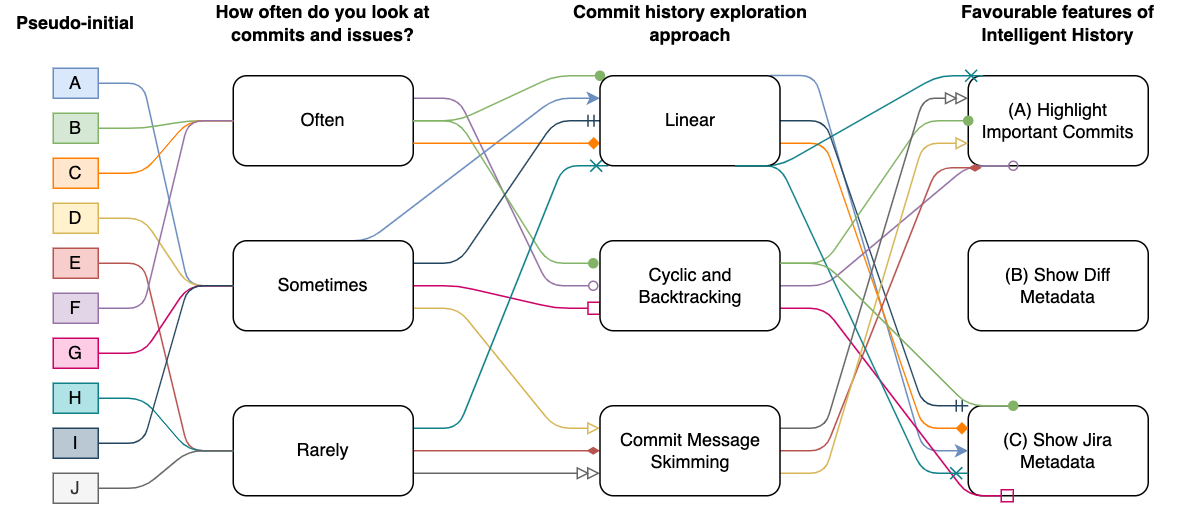
\includegraphics[width=12cm]{./images/flow-chart-ind.png}
  \caption{
    The relationship between how often a participant looks at commits and issues, 
    the approach they exhibited to exploring commit history overall, 
    and the feature of Intelligent History they were most partial to.
  }
  \label{fig:Flow-Chart-Individual}
\end{figure}

\begin{figure}[h]
  \centering
  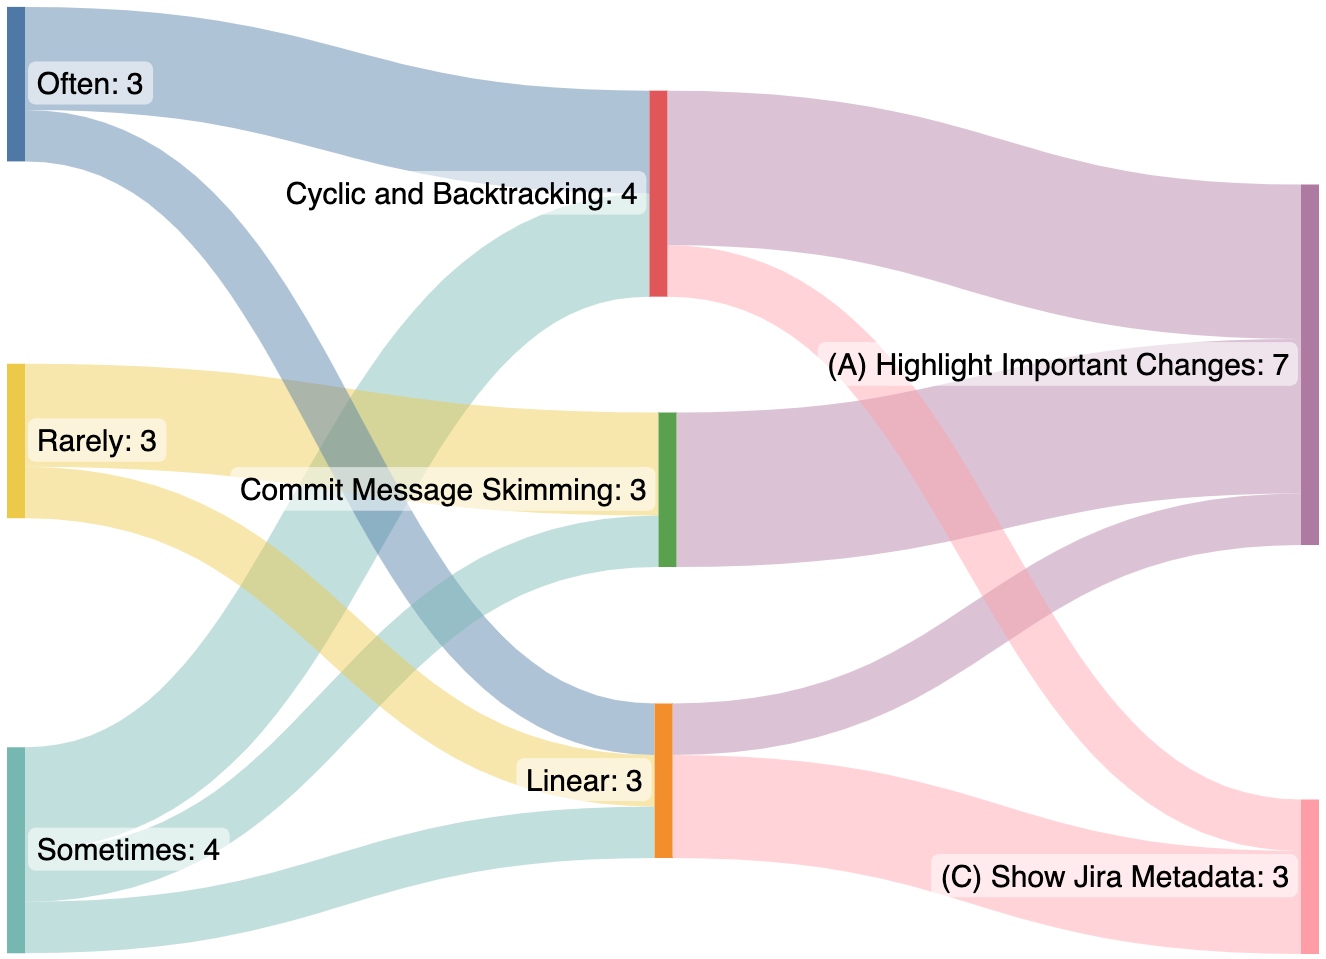
\includegraphics[width=8cm]{./images/flow-chart-aggr.png}
  \caption{
    An aggregation of the participants that fall into each of the categories from \autoref{fig:Flow-Chart-Individual} and \autoref{tab:Flow-Chart-Tabular}
  }
  \label{fig:Flow-Chart-Aggregate}
\end{figure}

Over half of the participants, 6 out of 10, preferred feature (\feature{1}) from Intelligent History the most,
whereas the other 4 participants preferred feature (\feature{3}).
Notably, all 5 of the participants who received question set A to answer with Intelligent History 
responded most positively to commit history highlighting in (\feature{1}) as a feature \participants{BDFHJ}, 
whereas 4 out of the 5 participants who received question set B to answer with Intelligent History 
responded most positively to gaining quick access to Jira issue information within the \entity{IDE} in (\feature{3}) as a feature \participants{ACGI}.
This signifies some degree of correlation between the question set and the participants' most preferred features of Intelligent History.

None of the participants chose feature (\feature{2}), though we anticipated this outcome as (\feature{2}) 
was provided to give the user context as to how Intelligent History highlights commits in (\feature{1}).
Of the 3 participants who stated that they often look at commits and issues, none demonstrated \textit{commit message skimming} 
as a strategy for exploring commit history.
Similarly, of the 3 participants who rarely look at commits and issues, none of them employed a commit history exploration approach 
that could be described as \textit{cyclic and backtracking}.
There does not appear to be any concrete associations between the background of a participant with regard to looking at commits and issues,
and their exhibited approach to exploring commit history.

On the relationship between the commit history exploration approach a participant exhibited and their preferred feature from Intelligent History,
3 out of 4 participants who demonstrated a \textit{cyclic and backtracking} approach expressed preference for (\feature{1}),
while all 3 participants who exhibited a \textit{commit message skimming} strategy were most partial to (\feature{3}).

\begin{landscape}
  \begin{table}
    \footnotesize
    \caption{
      A tabular form of \autoref{fig:Flow-Chart-Individual}.
    }
    \centering
    \begin{tabular}{@{}c|ccl@{}}
      \toprule
      \textbf{Pseudo-initial} & \textbf{\begin{tabular}[c]{@{}c@{}}How often do you look\\ at commits and issues?\end{tabular}} & \textbf{\begin{tabular}[c]{@{}c@{}}Commit history\\ exploration approach\end{tabular}} & \multicolumn{1}{c}{\textbf{\begin{tabular}[c]{@{}c@{}}Favourable feature of\\ Intelligent History\end{tabular}}} \\ \midrule
      A                       & Sometimes                                                                                       & Cyclic and Backtracking                                                                & (\feature{3}) Show Jira Metadata                                                                                           \\ \midrule
      B                       & Often                                                                                           & Cyclic and Backtracking                                                                & (\feature{1}) Highlight Important Changes                                                                                  \\ \midrule
      C                       & Often                                                                                           & Linear                                                                                 & (\feature{3}) Show Jira Metadata                                                                                           \\ \midrule
      D                       & Sometimes                                                                                       & Commit Message Skimming                                                                & (\feature{1}) Highlight Important Changes                                                                                  \\ \midrule
      E                       & Rarely                                                                                          & Commit Message Skimming                                                                & (\feature{1}) Highlight Important Changes                                                                                  \\ \midrule
      F                       & Often                                                                                           & Cyclic and Backtracking                                                                & (\feature{1}) Highlight Important Changes                                                                                  \\ \midrule
      G                       & Sometimes                                                                                       & Cyclic and Backtracking                                                                & (\feature{3}) Show Jira Metadata                                                                                           \\ \midrule
      H                       & Rarely                                                                                          & Linear                                                                                 & (\feature{1}) Highlight Important Changes                                                                                  \\ \midrule
      I                       & Sometimes                                                                                       & Linear                                                                                 & (\feature{3}) Show Jira Metadata                                                                                           \\ \midrule
      J                       & Rarely                                                                                          & Commit Message Skimming                                                                & (\feature{1}) Highlight Important Changes                                                                                  \\ \bottomrule
    \end{tabular}
    \label{tab:Flow-Chart-Tabular}
  \end{table}
\end{landscape}

\subsubsection{Breadth and Contextualization}

We anticipated question B1 to require the most application switching between the \entity{IDE} 
and browser and to have the highest number of mean Jira issues viewed.
This is because B1 requires participants to examine the diffs of commits to ensure they consist of source code changes 
that comply with the criteria of improving some functionality or behaviour in the \class{StreamsBuilder} class.
Participants were also asked to justify their answer by finding supporting evidence for the commit author's intent behind their change.

The participant group who did not use Intelligent History with B1 had a mean number of application switches of 2.0 (see \autoref{tab:Results-Quantitative-BA}),
while the group who did use Intelligent History with B1 had a mean number of application switches of 0.8 (see \autoref{tab:Results-Quantitative-AB}).
The group who did not use Intelligent History with B1 viewed a mean of 2.0 Jira issues (see \autoref{tab:Results-Quantitative-BA}),
while the group who did use Intelligent History with B1 viewed a mean of 3.2 Jira issues (see \autoref{tab:Results-Quantitative-AB}).
We observe that participants who used Intelligent History for locating meaningful source code changes and finding the code rationale behind the changes
were able to view more Jira issues with slightly less application switches than participants who did not use Intelligent History for the same task.

Coincidentally, 4 of the 5 participants from the group that answered question set B with 
Intelligent History actually favoured feature (\feature{3}) \textit{Show Jira Metadata} \participants{ACGI}.
Participant \participant{A} commented:

\begin{quote}
  I thought that the Jira integration was very helpful because you don’t have to go to Jira to look at all the stuff and deal with Jira. 
  It’s [the issues] just in the \entity{IDE} which is nice; it’s [the plugin] quick and fast.
\end{quote}

Participant \participant{I} mentioned:

\begin{quote}
  Without the plugin, it was a little more annoying and time-consuming opening up the browser, 
  looking for all of the issues, 
  whereas with the plugin, 
  it was already there [in the \entity{IDE}] and I can just take a quick look and see if it [the commit] 
  might be relevant and I can take a deeper look if needed.
\end{quote}

Of the 4 participants who favoured (\feature{3}), none demonstrated a commit message skimming approach to exploring commit history in the user study.
Only 1 of the participants reported looking at commits and issues often \participants{C},
while 3 participants reported sometimes \participants{AGI}.
Perhaps unsurprisingly, none of the participants who favoured (\feature{3}) reported looking at commits and issues rarely.

While we observed there to be some notable difference in the group that used Intelligent History for question B1 and the group that did not use Intelligent History for the same question,
there is less notable difference with question B2.
Hence, we find that the primary question responsible for this bias is question B1.
Given the nature of B1, we find direct integration of Jira issue information within the \entity{IDE} 
to be useful for broad search and exploration of a commit history.
As participant \participant{E} stated:
``\textit{[The Jira issue integration] helps you contextualize the code change in a commit really quick.}''
However, direct issue integration is potentially less useful for those with an approach based on skimming commit messages.

\subsubsection{Issue Content and Presentation}

We found 2 participants mentioned a preference to see the full Jira issue information contextualized in the browser interface \participants{DF}.
While participant \participant{F} mentioned that they were accustomed to viewing Jira issues in the browser,
participant \participant{D} stated that they had a preference to view all items associated with a Jira issue, including all linked issues and pull requests:
``\textit{When I’m looking at a Jira ticket, I look at everything associated with the ticket to try to get a much broader context.}''
On the other hand,
participant \participant{E} stated that they did not look at parts of an issue beyond the description and a few comments:
``\textit{I wouldn’t bother that much with looking at the issue for other things like discussion, other than the description and perhaps the last two comments, 
I wouldn’t look much further than that}.''
We found there may be some limitations related to \emph{what} information was presented in the integrated view of the Jira issue in the \entity{IDE}
and the personal preferences and habits of the user.

Similar in sentiment, participant \participant{G}, who favoured (\feature{3}), noted the hyperlinking of Jira issues for each commit
was most helpful to them in the user study.
\participant{G} observed that since some of the Jira issues included code fragments, it was difficult to read them in the \entity{IDE}.
This indicates the presentation of the issue information may be an impediment to its utility.

\begin{summary}[RQ3]
  Direct integration of issue information can help software developers contextualize source code changes 
  and access the information in more issues than without,
  particularly when searching for interesting or meaningful changes across a file's commit history.
  However, the utility of direct integration of issue information is dependent on users' preferences preferences and habits 
  with regard to the content they prefer to see from issues and how they would like them to be presented.
\end{summary}

%%%%%%%%%%%%%%%%%%%%%%%%%%%%%%%%%%%%%%%%%%%%%%%%%%%%%%%%%%%%%%%%%%%%%%

\section{Threats to Validity}

\subsection{Construct Validity}

The size of the question sets we asked is a threat to construct validity.
Due to the laboratory setting of the user study and the time estimated for participants to perform environment setup,
be introduced to the Apache Kafka project, Jira, the IntelliJ IDEA IDE, and the Intelligent History plugin,
we restricted the number of questions asked to account for a reasonable total estimated session time.
We formulated small sets of questions to relieve participants from a time limit 
and give them the freedom to explore the commit histories, inspect individual commits, and read Jira issues at their own pace.
Although the small quantity of questions allowed us to observe the participants closely for each information-finding question,
we risk the ability to observe the consistency of the participants' commit history exploration strategies
across larger sets of questions to use without and with Intelligent History.

The realism of the questions we asked also threatens construct validity.
The questions we formulated in A1, A2, B1, and B2 and the commit history exploration 
they require may not be reflective of the tasks software developers perform in practice.
These questions or the activities required to answer them would typically be
asked or performed in the context of a larger goal, 
such as tracing the origin of a bug or seeking the introduction of a specific feature.

\subsection{Internal Validity}

The presence of an observer in the user study sessions means the participants' behaviour, opinions, 
and feedback about the Intelligent History plugin are subject to the Hawthorne effect,
which threatens internal validity.
The presence of an observer could have caused participants to deviate from their regular work habits 
as the participants might have formed an expectation about how to behave or explore the commit history.
We attempted to mitigate this effect by minimizing observer interjections during the sessions, 
though prior to the study, participants were encouraged to think aloud to describe their strategies 
to finding the information necessary to answer the questions.
We also provided participants with the opportunity to self-report, clarify their actions, 
and provide feedback on their experience with participating in the user study during the semi-structured interview
portion of the user study.

The introduction of the Intelligent History plugin to the participant could be a threat to internal validity.
After being introduced to the features of Intelligent History, 
the participant could be biased to use or conduct themselves in the study a certain way.
For example, toggling feature (\feature{1}) \textit{Highlight Important Changes} 
results in highlighting the commits in a commit history to distinguish less important commits from potentially more important commits.
If we initially introduced Intelligent History to a participant for their first question set,
and asked the participants to work on a second question set without Intelligent History,
they may have tried to answer the questions in the same way they would have if they had access to Intelligent History.
Consequently, in the semi-structured interview part of the study, 
participants may have felt biased to feel a certain way about the plugin.

We tried to mitigate bias in how a participant expects to use Intelligent History 
and the utility of Intelligent History to a particular question set 
by alternating the order of the questions each participant received 
and fixing the use of the plugin to the second question set that each participant receives.
By providing each participant with a different set of questions to answer with 
and without Intelligent History respectively,
we also mitigate the threat to internal validity of a participant having 
exposure to the same questions prior to using Intelligent History.
Though the participants might have felt biased after using the plugin,
we would still be able to retain and collect data about how the participant approached 
exploring the commit history and answering the questions without being made aware of the plugin's features initially.

The experience of the participants with regard to having worked on a project that uses an issue tracking system 
and closely associating issues to commits impacts internal validity.
We tried to mitigate the impact of participant experience on internal validity by formulating questions 
that would require participants to justify their answers using source code and Jira issue information to
encourage participants to view Jira issues.

\subsection{External Validity}

The sample size of 10 participants affects the generalizability of our results and is a threat to external validity.
Collecting data for a larger sample size may lead to more robust conclusions about the relationship 
between a developer's experience with looking at issues and commits,
the commit history exploration strategy or strategies they employ, 
and the aspects of Intelligent History they found to be most useful.
Nevertheless, a strength of our participant pool is representation. 
We obtained samples from 4 students and 6 professional developers from different companies,
representing a combination of participants from academia and industry.

A field study to investigate and evaluate the performance of the approaches in Intelligent History might also be needed to improve generalizability.
Rather than designing sets of questions pertaining to the commit history and issues available in one open-source repository,
which was Apache Kafka in our user study,
a field study to investigate how developers explore commit history with and without Intelligent History in the wild 
could lead to a more robust model for determining non-essential and essential commits,
as well as gain a deeper understanding of how often developers use issues from an issue tracking system and how they prioritize the information in an issue.

%%%%%%%%%%%%%%%%%%%%%%%%%%%%%%%%%%%%%%%%%%%%%%%%%%%%%%%%%%%%%%%%%%%%%%
\endinput

Any text after an \endinput is ignored.
You could put scraps here or things in progress.
\chapter{Discussion}
\label{ch:Discussion}

In this chapter, we discuss the implications of our findings,
potential improvements to our approach, and the threats to validity of our work.

%%%%%%%%%%%%%%%%%%%%%%%%%%%%%%%%%%%%%%%%%%%%%%%%%%%%%%%%%%%%%%%%%%%%%%

\section{Using Regular Expressions to Improve Software History Exploration}

Although we formulated a fixed set of patterns specific to Java, \dots \FIXME{Consider moving this to a section on suggestions for future work? Comment on potential for user-defined patterns.}

Making the analysis of important comments more sensitive to task and context.

%%%%%%%%%%%%%%%%%%%%%%%%%%%%%%%%%%%%%%%%%%%%%%%%%%%%%%%%%%%%%%%%%%%%%%

\section{Improving Usability of Issues for Code Rationale Information}

%%%%%%%%%%%%%%%%%%%%%%%%%%%%%%%%%%%%%%%%%%%%%%%%%%%%%%%%%%%%%%%%%%%%%%

\section{Task-Sensitivity}

%%%%%%%%%%%%%%%%%%%%%%%%%%%%%%%%%%%%%%%%%%%%%%%%%%%%%%%%%%%%%%%%%%%%%%

\section{Limitations and Future Work}

%%%%%%%%%%%%%%%%%%%%%%%%%%%%%%%%%%%%%%%%%%%%%%%%%%%%%%%%%%%%%%%%%%%%%%

\section{Threats to Validity}

There are a number of aspects of this user study that impact the validity of our results.
Firstly, since the participants were observed throughout the study by the interviewer, the participants' behaviour, opinions, and feedback about the Intelligent History plugin are subject to the Hawthorne effect.
We attempted to mitigate bias in how a participant expects to use Intelligent History and the applicability of Intelligent History to any particular question set 
by alternating the order of the questions each participant received and 
fixing the use of the plugin to the second question set that each participant receives.

The experience of the participants with regard to experience in working in a project that uses an issue tracking system (\entity{ITS}) and closely associating issues to commits impacts internal validity.
We tried to mitigate the impact of participant experience on internal validity by formulating questions that would require participants to justify their answers using source code and Jira issue information to
encourage participants to view Jira issues.

The limited participant size of 10 participants and the controlled experiment setting of the user study affects external validity.

%%%%%%%%%%%%%%%%%%%%%%%%%%%%%%%%%%%%%%%%%%%%%%%%%%%%%%%%%%%%%%%%%%%%%%
\endinput

Any text after an \endinput is ignored.
You could put scraps here or things in progress.
\chapter{Conclusion}
\label{ch:Conclusion}

In this thesis, our goal was to \dots
To this end, \dots

%    3. Notes
%    4. Footnotes

%    5. Bibliography
\begin{singlespace}
\raggedright
\bibliographystyle{abbrvnat}
\bibliography{biblio}
\end{singlespace}

\appendix
%    6. Appendices (including copies of all required UBC Research
%       Ethics Board's Certificates of Approval)
%\include{reb-coa}	% pdfpages is useful here
\chapter{Supporting Materials}

%%%%%%%%%%%%%%%%%%%%%%%%%%%%%%%%%%%%%%%%%%%%%%%%%%%%%%%%%%%%%%%%%%%%%%
\section{Briefing and Setup Instructions}
\label{sec:Briefing-and-Setup}

\subsection{Briefing}
\label{subsec:Briefing}

Apache Kafka is an event streaming platform used to collect, process, and store streaming event data that has no discrete beginning or end, \eg real-time stock trades and social media feeds. 
As part of Kafka’s contribution guidelines, a commit’s title/subject is usually of the form ``KAFKA-XXXX: Title,'' where ``KAFKA-XXXX'' is the relevant Jira issue ID and ``Title'' may be the Jira’s title or a more specific title describing the pull request itself. 
For trivial cases where a Jira issue is not required, ``MINOR:'' or ``HOTFIX:'' is used as the commit’s title prefix.

In this study, you will be exploring two Java classes and their commit histories from the Kafka project and answering a series of questions in a semi-structured interview format. The process of finding the answers to these questions can involve reading the commit messages for commits and visiting the relevant Jira issue on Apache’s Jira instance:
\url{https://issues.apache.org/jira/browse/KAFKA-XXXX}.

You may also see the acronym ``KIP'' referenced in some commits or Jira issues in Kafka. You may use and reference KIPs in your exploration and answers. These are Kafka Improvement Proposals (\entity{KIP}s) and can be found at: 
\url{https://cwiki.apache.org/confluence/display/kafka/kafka+improvement+proposals}.

\subsection{Setup Instructions}
\label{sec:Setup-Instructions}

\begin{enumerate}
    \item Install IntelliJ IDEA, either Community (free) or Ultimate edition (if you already have a license). See: \url{https://www.jetbrains.com/idea}. If you already have IntelliJ installed, please confirm the version number. The version must be 2022.1 or greater, which you can verify by navigating to the top bar  ``Help'' → ``About'' (Windows) or top bar → ``IntelliJ IDEA'' → ``About IntelliJ IDEA'' (Mac).
    \item Clone the Apache Kafka repository (roughly 200 MB on disk) or you can request the co-investigator to provide a ZIP of the repository: 
    
    \begin{center}
        \code{git clone --single-branch --branch trunk https://github.com/apache/kafka.git}
    \end{center}

    \item Open the Kafka project in IntelliJ: ``File'' → ``Open''
    \item To install the plugin, download \code{Intelligent.History-1.0.0.zip} at: \url{https://github.com/Alison-Li/intelligent-history/releases/tag/v1.0.0-eval}. Go to “Settings/Preferences” → ``Plugins'' → Gear Icon → ``Install Plugin from Disk\dots''
    \item For the task involving the plugin: Go to ``Settings/Preferences'' → ``Tools'' → ``Intelligent History'' to configure the Jira settings. Alternatively, go to “Settings/Preferences’ → type ``Intelligent History'' in the search field to look for the plugin settings. The co-investigator will provide you with the information needed to fill in the fields.
\end{enumerate}

%%%%%%%%%%%%%%%%%%%%%%%%%%%%%%%%%%%%%%%%%%%%%%%%%%%%%%%%%%%%%%%%%%%%%%
\section{Question Sets}

\subsection{Set A}
\label{subsec:Question-Set-A}

Open and examine the following Java class from the Apache Kafka repository:
\class{Topology.java}\footnote{\url{https://github.com/apache/kafka/blob/trunk/streams/src/main/java/org/apache/kafka/streams/Topology.java}}

\begin{enumerate}
    \item Using commit message information and/or Jira issue information, can you describe the motivation behind why the code segment on lines 717 to 722 was introduced and the benefit to the user of the Kafka \entity{API}?
    \item There are several overloaded methods called \code{addSink} in this class. In your own words, can you describe in what context were these overloaded methods introduced to this class?
    \item What was the motivation behind the most recent commit (\commit{fbe7fb94}) made to this class?
\end{enumerate}

\subsection{Set B}
\label{subsec:Question-Set-B}

Open and examine the following Java class from the Apache Kafka repository:
\class{StreamsBuilder.java}\footnote{\url{https://github.com/apache/kafka/blob/trunk/streams/src/main/java/org/apache/kafka/streams/StreamsBuilder.java}}

\begin{enumerate}
    \item Can you find two commits that represent changes that were introduced to improve some functionality in this class and justify why you chose them? The changes can not be cosmetic such as removing repeated words, removing deprecated code, or adding/modifying/removing documentation and comments. 
    \item Why is the \code{build} method in this class overloaded? Specifically, why was the overloaded build method in lines 623 to 630 introduced?
\end{enumerate}

%%%%%%%%%%%%%%%%%%%%%%%%%%%%%%%%%%%%%%%%%%%%%%%%%%%%%%%%%%%%%%%%%%%%%%
\section{Interview Questions}
\label{sec:Interview-Questions}

\begin{enumerate}
    \item How many years of software development experience do you have, both professionally and non-professionally?
    \item In your development experience, have you often looked at commits and the issues associated with them (e.g. GitHub issues/pull requests, Jira issues, Bugzilla, etc.)?
        \begin{enumerate}
            \item In what scenarios or kinds of tasks do you typically look at commits and issues?
        \end{enumerate}
    \item What types of code changes or content in diffs do you think are less useful or more useful when trying to understand why a developer wrote code a certain way or made a particular change? 
    \item Are there any particular contexts or examples from your experience you can think of?
    \item For the task involving use of the plugin, which features did you find helpful/unhelpful to your exploration?
    \item Are there any comments or feedback you would like to provide?
\end{enumerate}

%%%%%%%%%%%%%%%%%%%%%%%%%%%%%%%%%%%%%%%%%%%%%%%%%%%%%%%%%%%%%%%%%%%%%%
\endinput

This would be any supporting material not central to the dissertation.
For example:
\begin{itemize}
\item additional details of methodology and/or data;
\item diagrams of specialized equipment developed.;
\item copies of questionnaires and survey instruments.
\end{itemize}

\backmatter
%    7. Index
% See the makeindex package: the following page provides a quick overview
% <http://www.image.ufl.edu/help/latex/latex_indexes.shtml>


\end{document}
